\documentclass[compress]{beamer}
\usepackage{ifthen,verbatim}

\newcommand{\isnote}{}
\xdefinecolor{lightyellow}{rgb}{1.,1.,0.25}
\xdefinecolor{darkblue}{rgb}{0.1,0.1,0.7}

%% Uncomment this to get annotations
%% \def\notes{\addtocounter{page}{-1}
%%            \renewcommand{\isnote}{*}
%% 	   \beamertemplateshadingbackground{lightyellow}{white}
%%            \begin{frame}
%%            \frametitle{Notes for the previous page (page \insertpagenumber)}
%%            \itemize}
%% \def\endnotes{\enditemize
%% 	      \end{frame}
%%               \beamertemplateshadingbackground{white}{white}
%%               \renewcommand{\isnote}{}}

%% Uncomment this to not get annotations
\def\notes{\comment}
\def\endnotes{\endcomment}

\setbeamertemplate{navigation symbols}{}
\setbeamertemplate{headline}{\mbox{ } \hfill
\begin{minipage}{5.5 cm}
\vspace{-0.75 cm} \small
\end{minipage} \hfill
\begin{minipage}{4.5 cm}
\vspace{-0.75 cm} \small
\begin{flushright}
\ifthenelse{\equal{\insertpagenumber}{1}}{}{Jim Pivarski \hspace{0.2 cm} \insertpagenumber\isnote/\pageref{numpages}}
\end{flushright}
\end{minipage}\mbox{\hspace{0.2 cm}}\includegraphics[height=1 cm]{../cmslogo} \hspace{0.1 cm} \includegraphics[height=1 cm]{../tamulogo} \hspace{0.01 cm} \vspace{-1.05 cm}}

\newcommand{\s}[1]{{\mbox{\scriptsize #1}}}

\begin{document}
\begin{frame}
\vfill
\begin{center}
\textcolor{darkblue}{\Large Search for Dimuon Resonances in ``Lepton Jets''}

\vfill
\begin{columns}
\column{0.3\linewidth}
\begin{center}
\large
\textcolor{darkblue}{\it Jim Pivarski}

Alexei Safonov

Aysen Tatarinov

\vspace{0.5 cm}
\scriptsize
{\it Texas A\&M University}

\vspace{0.5 cm}
\normalsize
20 January, 2011
\end{center}

\column{0.35\linewidth}
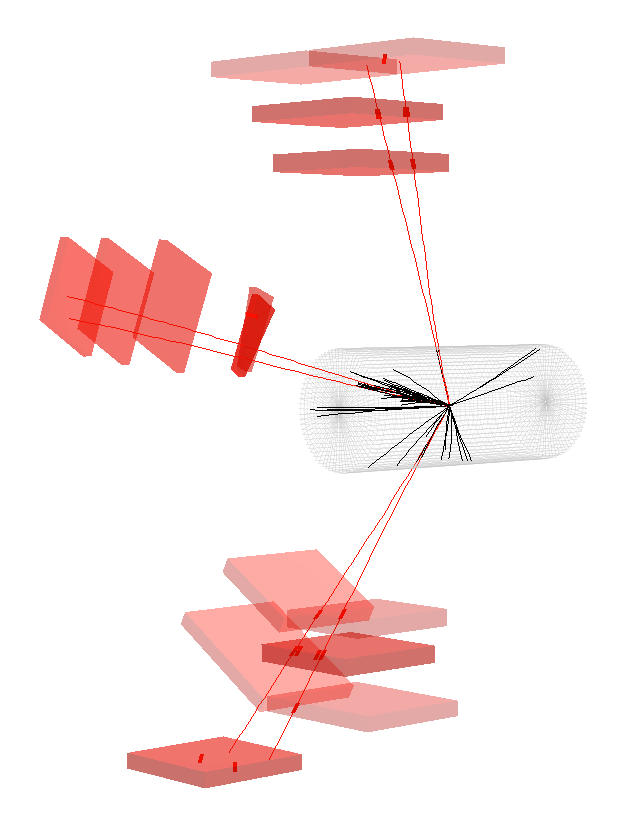
\includegraphics[width=\linewidth]{eventdisplay_3d.png}
\end{columns}

\end{center}
\end{frame}

%% \begin{notes}
%% \item This is the annotated version of my talk.
%% \item If you want the version that I am presenting, download the one
%% labeled ``slides'' on Indico (or just ignore these yellow pages).
%% \item The annotated version is provided for extra detail and a written
%% record of comments that I intend to make orally.
%% \item Yellow notes refer to the content on the {\it previous} page.
%% \item All other slides are identical for the two versions.
%% \end{notes}

\small

\section{Introduction}

\begin{frame}
\frametitle{\only<1>{Generic phenomenology (sketch)}\only<2>{Dark SUSY example}\only<3>{NMSSM Higgs example}}
\begin{center}
\only<1>{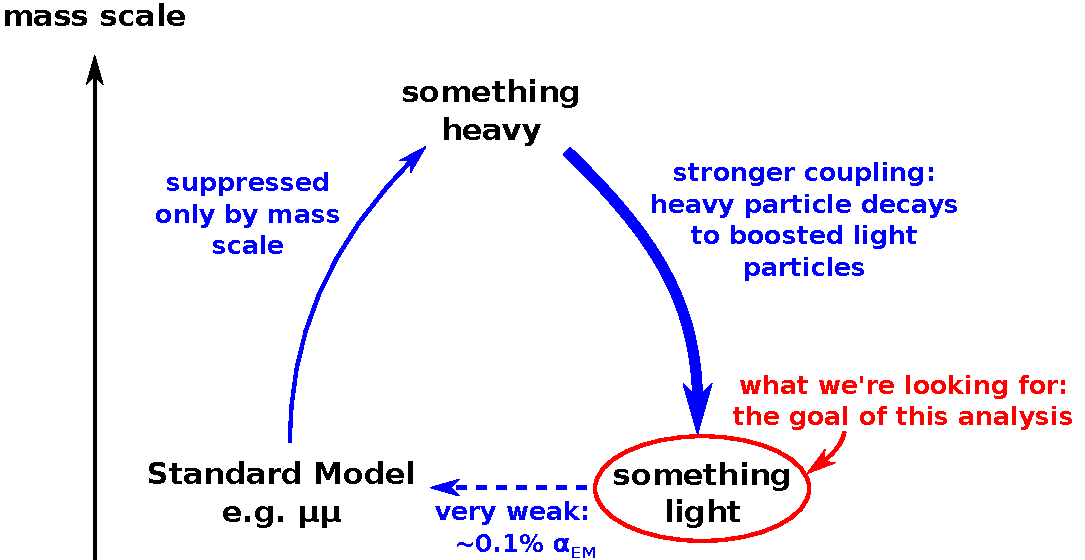
\includegraphics[width=0.9\linewidth]{basic_picture.pdf}}
\only<2>{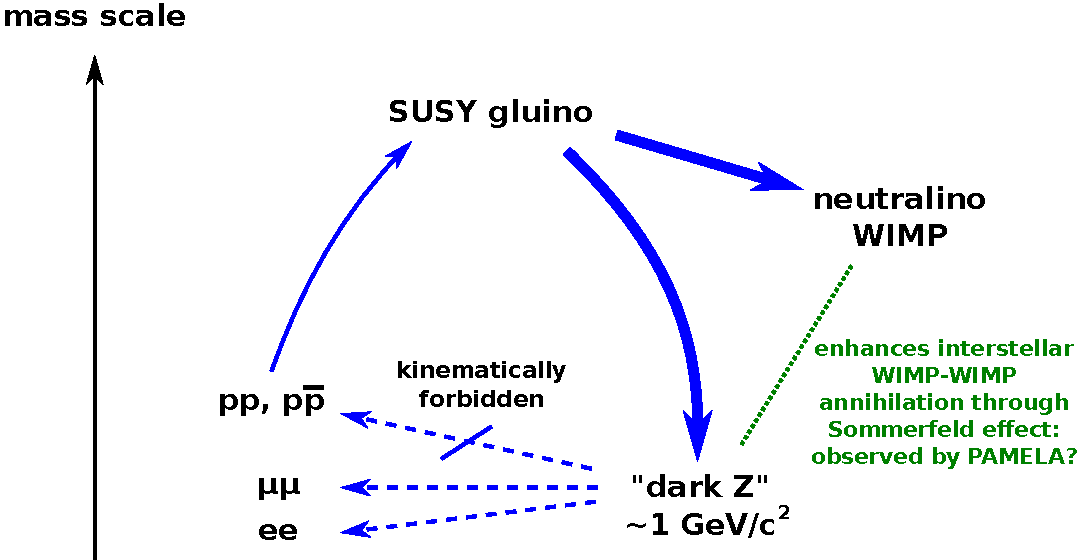
\includegraphics[width=0.9\linewidth]{basic_picture2.pdf}}
\only<3>{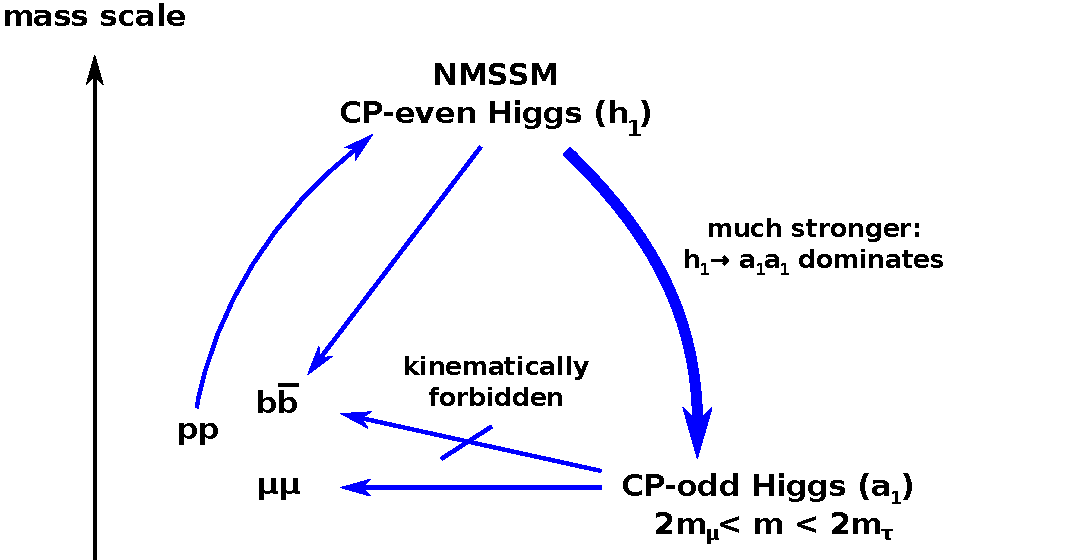
\includegraphics[width=0.9\linewidth]{basic_picture3.pdf}}
\end{center}

\begin{itemize}
\item \only<1>{Hidden-valley picture: predicts new low-mass, high-momentum particles decaying to Standard Model pairs like $\mu\mu$}\only<2>{Sub-class motivated by PAMELA positron excess (and lack of antiproton excess) when interpreted as WIMP-WIMP annihilation}\only<3>{A region of NMSSM parameter space allows the Higgs to escape LEP limits by decaying to lighter Higgs bosons rather than $b\bar{b}$, $\tau^+\tau^-$, etc.}
\item<1,3> \only<1>{We want to maximize our sensitivity to ``something like this''}\only<3>{Same basic picture, same signature}
\end{itemize}
\end{frame}

\begin{frame}
\frametitle{Analysis strategy}
\begin{columns}
\column{0.55\linewidth}
Motivated by phenomenology:
\begin{itemize}
\item Hidden sector's spectrum is unknown, but weak coupling to
  the Standard Model implies that it predominantly passes through the lightest
  hidden state

\textcolor{darkblue}{$\longrightarrow$ search for low-mass dimuons}

\item Muon pairs may overlap, but cascades of light particles would
  be collimated in groups by their boost

\textcolor{darkblue}{$\longrightarrow$ first identify well-separated groups, then
  resolve combinatorics}

\item $\mathcal{B}(m_1 \to \mu\mu)$ is likely to be high, but not
  necessarily 100\%

\textcolor{darkblue}{$\longrightarrow$ look for muons, but neither
  require nor exclude other particles (e.g.\ by applying an isolation cut)}
\end{itemize}

\column{0.5\linewidth}
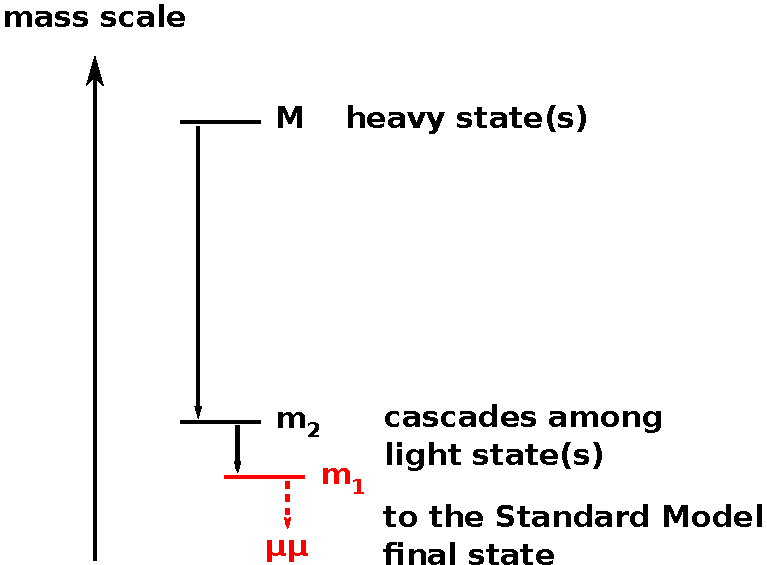
\includegraphics[width=\linewidth]{basic_picture4.pdf}

\begin{center}
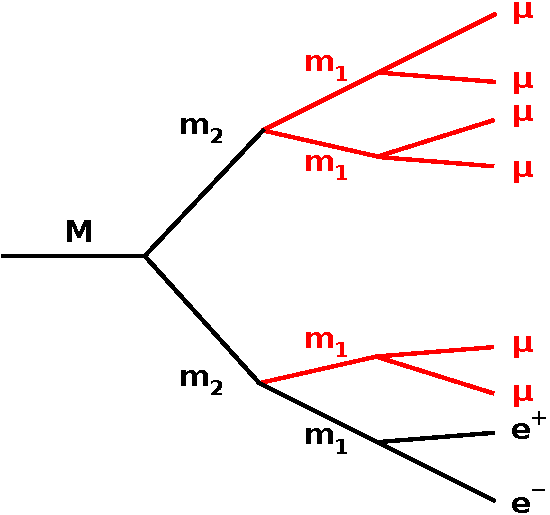
\includegraphics[width=0.7\linewidth]{basic_picture5.pdf}
\end{center}
\end{columns}
\end{frame}

\begin{frame}
\frametitle{Analysis strategy}
\begin{columns}
\column{0.57\linewidth}
\begin{itemize}
\item Unless the hidden spectrum has a very close degeneracy, the
  lightest state ($m_1$) will be on-shell

  \textcolor{darkblue}{\mbox{$\longrightarrow$ search for a resonance peak}}  % $^*$\hspace{-0.5 cm}}}

\item Groups of four or more muons represent $m_2 \to m_1 m_1$ cascades

  \textcolor{darkblue}{$\longrightarrow$ split them into the
      most consistent assignment of dimuon masses (assumes on-shell $m_1$)}

\item Different event topologies have different backgrounds

  \textcolor{darkblue}{$\longrightarrow$ partition signal region by
    number of collimated groups (``mu-jets'') and number of dimuons within each mu-jet}
\end{itemize}

\column{0.36\linewidth}
\vspace{0.1 cm}
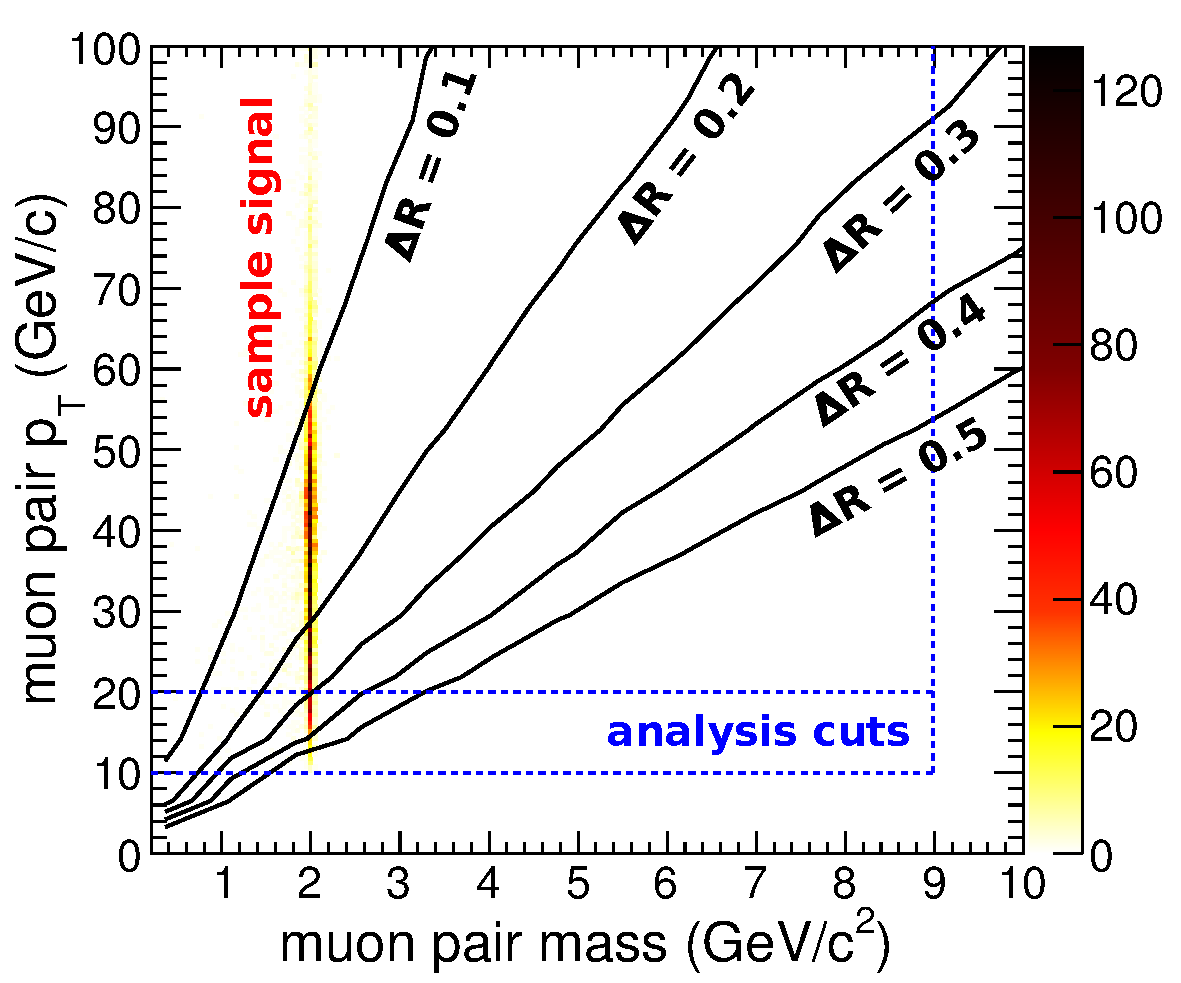
\includegraphics[width=\linewidth]{openingangle_with_signal.pdf}

\vspace{0.3 cm}
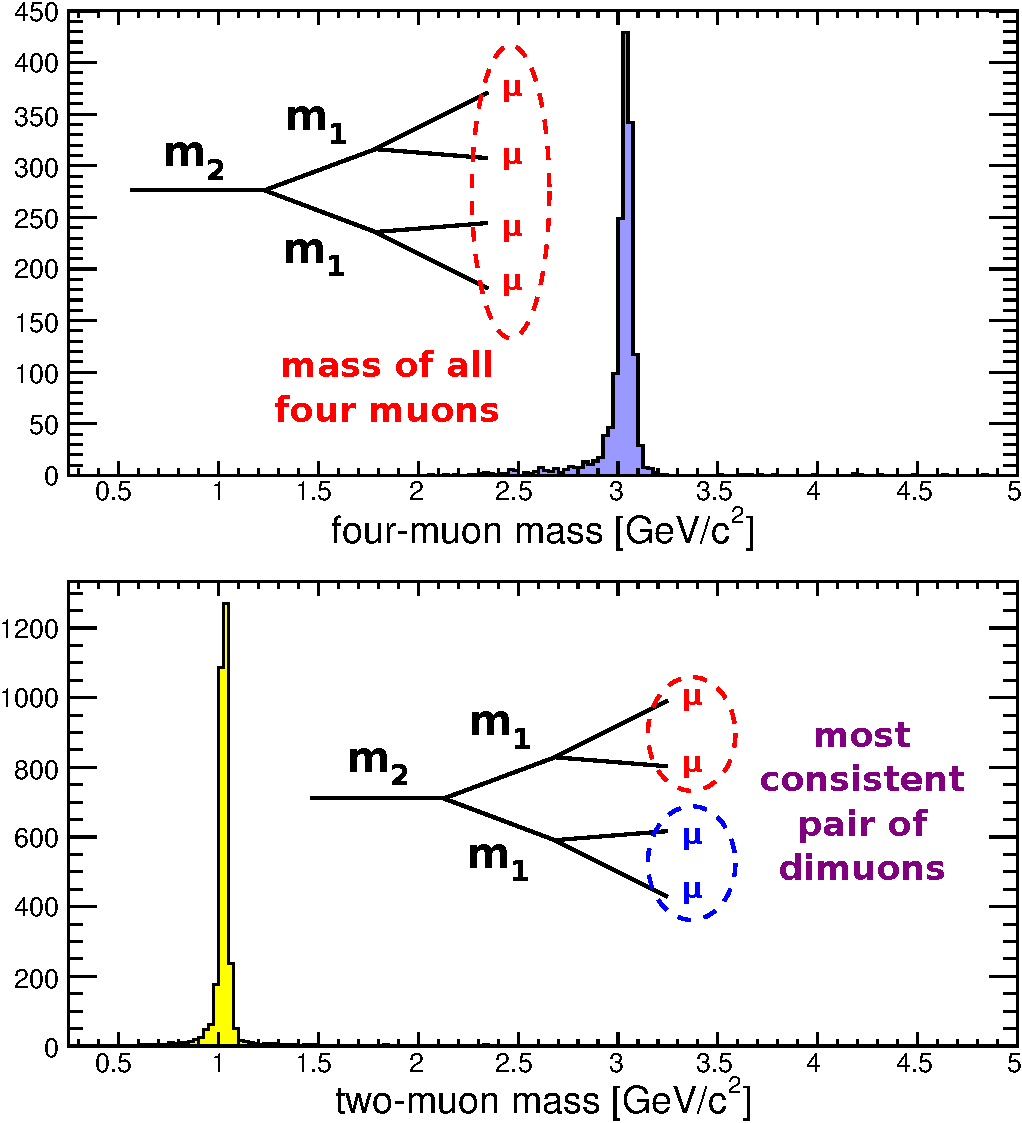
\includegraphics[width=\linewidth]{four-two-muon-mass.pdf}
\end{columns}

% \mbox{\textcolor{darkblue}{\scriptsize $^*$Also searched for non-resonant $m_2 \to m_1 m_1$ ($m_2 < 9$~GeV/$c^2$) in four-muon spectrum\hspace{-1 cm}}}
\end{frame}

\begin{frame}
\frametitle{Signal topologies}

\vspace{1 cm}
\hfill 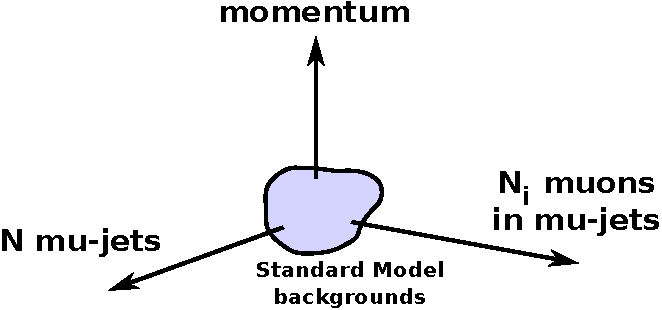
\includegraphics[width=0.5\linewidth]{signal_regions.pdf}

\vspace{-3.5 cm}
\begin{itemize}
\item \mbox{Look for new resonance in all channels that have small backgrounds\hspace{-0.5 cm}}

\item Any one of the following reduce \\ Standard Model backgrounds to $\mathcal{O}(1\mbox{ pb})$:
\begin{itemize}
\item $p_T \gtrsim 80$~GeV/$c$
\item $\ge 2$ mu-jets in an event
\item $\ge 4$ muons in a mu-jet
\end{itemize}
\item Define non-overlapping signal regions:
\end{itemize}

\vspace{-0.5 cm}
\begin{center}
\begin{minipage}{0.8\linewidth}
\scriptsize
\begin{enumerate}[(\alph{enumi})]
\item exactly one mu-jet per event
\begin{enumerate}[(\scriptsize \mbox{a}-\arabic{enumii})]
\item \scriptsize $p_T > 80$~GeV/$c$ mu-jet containing two muons \mbox{($m_1 \to 2\mu$)\hspace{-1 cm}}
\item \scriptsize any mu-jet containing four muons ($m_2 \to m_1 m_1 \to 4\mu$)
\item \scriptsize more than four
\end{enumerate}

\item two mu-jets per event
\begin{enumerate}[\scriptsize (b-\arabic{enumii})]
\item \scriptsize $2\mu$, $2\mu$ ($M \to m_1 m_1$, which is the NMSSM signature)
\item \scriptsize $2\mu$, $4\mu$ ($M \to m_1 m_2$)
\item \scriptsize $4\mu$, $4\mu$ ($M \to m_2 m_2$)
\item \scriptsize either has more than four
\end{enumerate}

\item \scriptsize more than two mu-jets per event
\end{enumerate}
\end{minipage}
\end{center}
\end{frame}

\begin{frame}
\frametitle{Signal extraction}

\begin{itemize}
\item Unlike jets, our signals have a well-defined but unknown mass
\begin{itemize}
\item all on-shell $m_1$ particles in an event have the same mass
\item backgrounds fill the space of dimuon masses more uniformly
\end{itemize}
\item Measure signal and backgrounds in a single ``fit with sidebands''
\begin{itemize}
\item topologies with $n$ dimuons per event form an $n$-dimensional
  space of observables
\item signal is a sharp peak somewhere along the diagonal
\item background distribution is a Cartesian product of shapes derived from data
\end{itemize}

\begin{center}
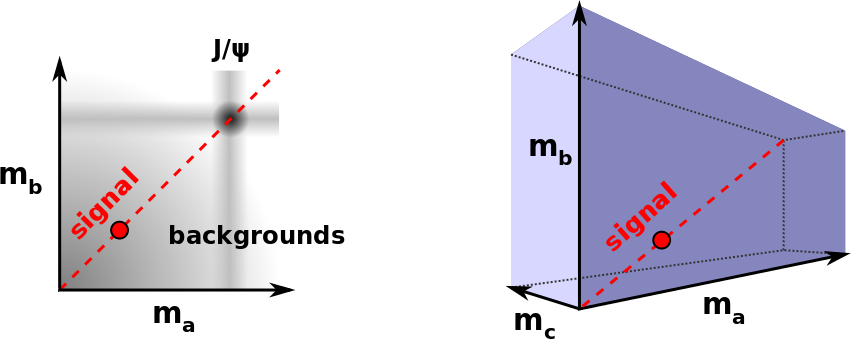
\includegraphics[width=0.9\linewidth]{diagonal.png}
\end{center}
\end{itemize}
\end{frame}

\begin{frame}
\frametitle{Outline for the rest of the talk}
\framesubtitle{In reverse historical order!}

\begin{itemize}\setlength{\itemsep}{0.5 cm}
\item Opening the box: results unblinded last weekend
\item Deriving the shape templates
\item Detector issues; acceptance and efficiency
\item Implications for benchmark models
\end{itemize}
%% \hspace{-0.83 cm} \textcolor{darkblue}{\Large Outline2}
\end{frame}

\section*{Opening the Box}
\begin{frame}

\vfill
\begin{center}
\Huge \textcolor{blue}{Opening the Box}
\end{center}

\vfill
\end{frame}

\begin{frame}
\frametitle{Results: all consistent with SM}

\begin{columns}
\column{0.5\linewidth}
\begin{tabular}{c p{0.85\linewidth}}
137 & events with a single, high-$p_T$ dimuon (SM-like distribution) \\
1 & event with a 4-$\mu$ mu-jet \\
11 & events with two 2-$\mu$ mu-jets \\
\textcolor{darkblue}{0} & \textcolor{darkblue}{events within 5$\sigma$ (detector \mbox{resolution}) of a 2-D diagonal} \\
\textcolor{darkblue}{0} & \textcolor{darkblue}{events with 3 or more dimuons}
\end{tabular}

\column{0.5\linewidth}
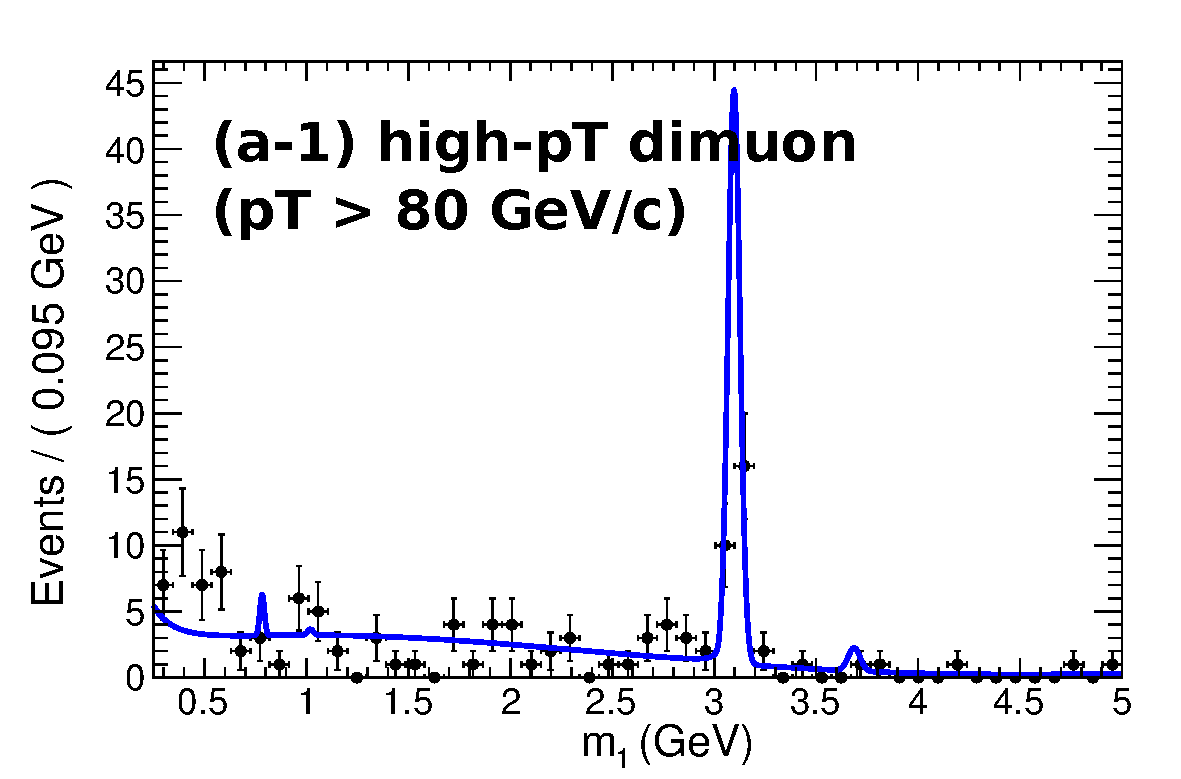
\includegraphics[width=\linewidth]{signal_a1_data-bkgpdf.pdf}
\end{columns}

\begin{columns}
\column{0.5\linewidth}
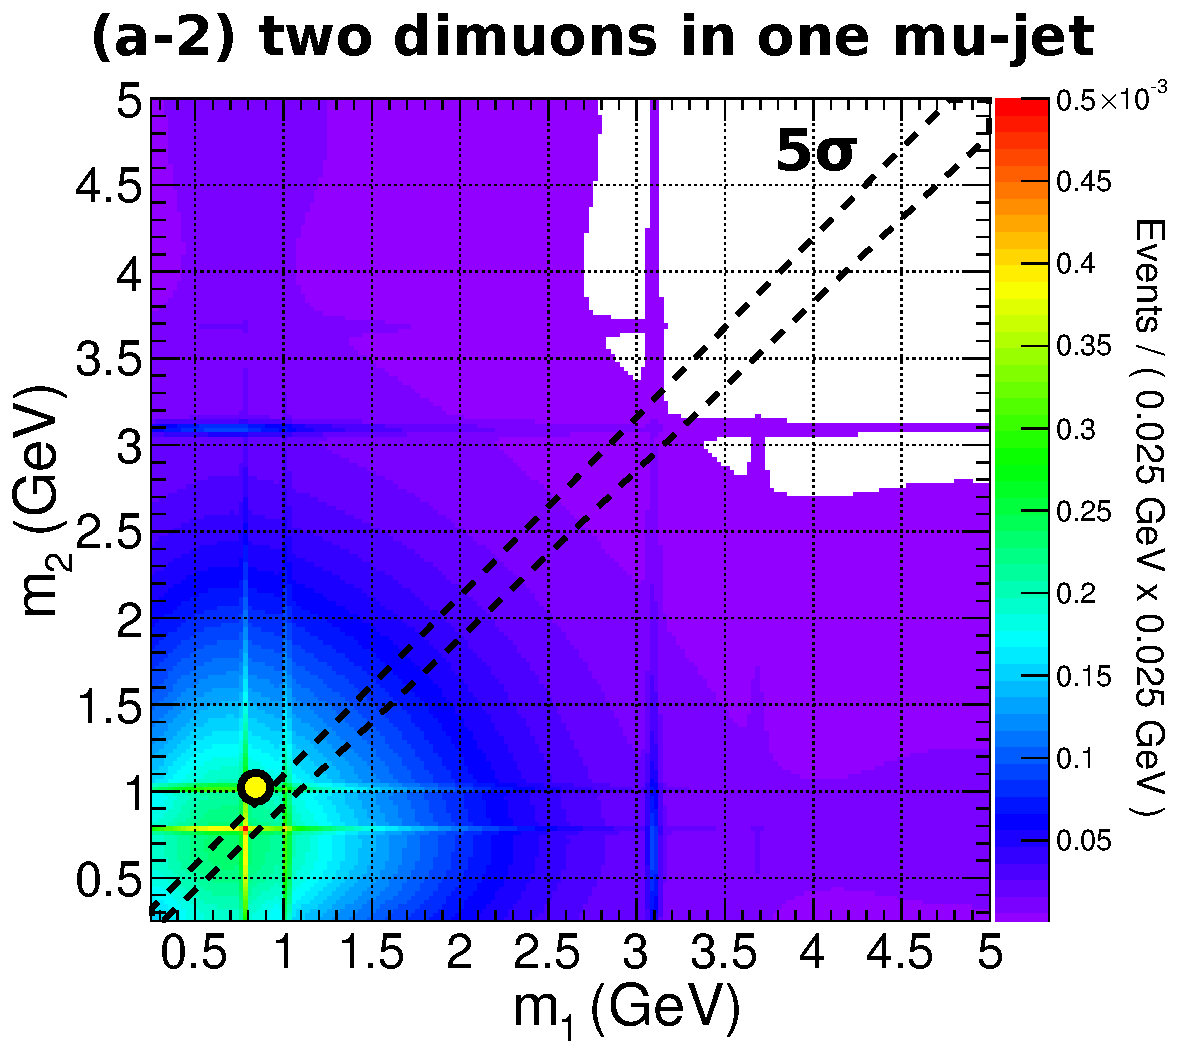
\includegraphics[width=\linewidth]{a2_2dpdf.pdf}

\column{0.5\linewidth}
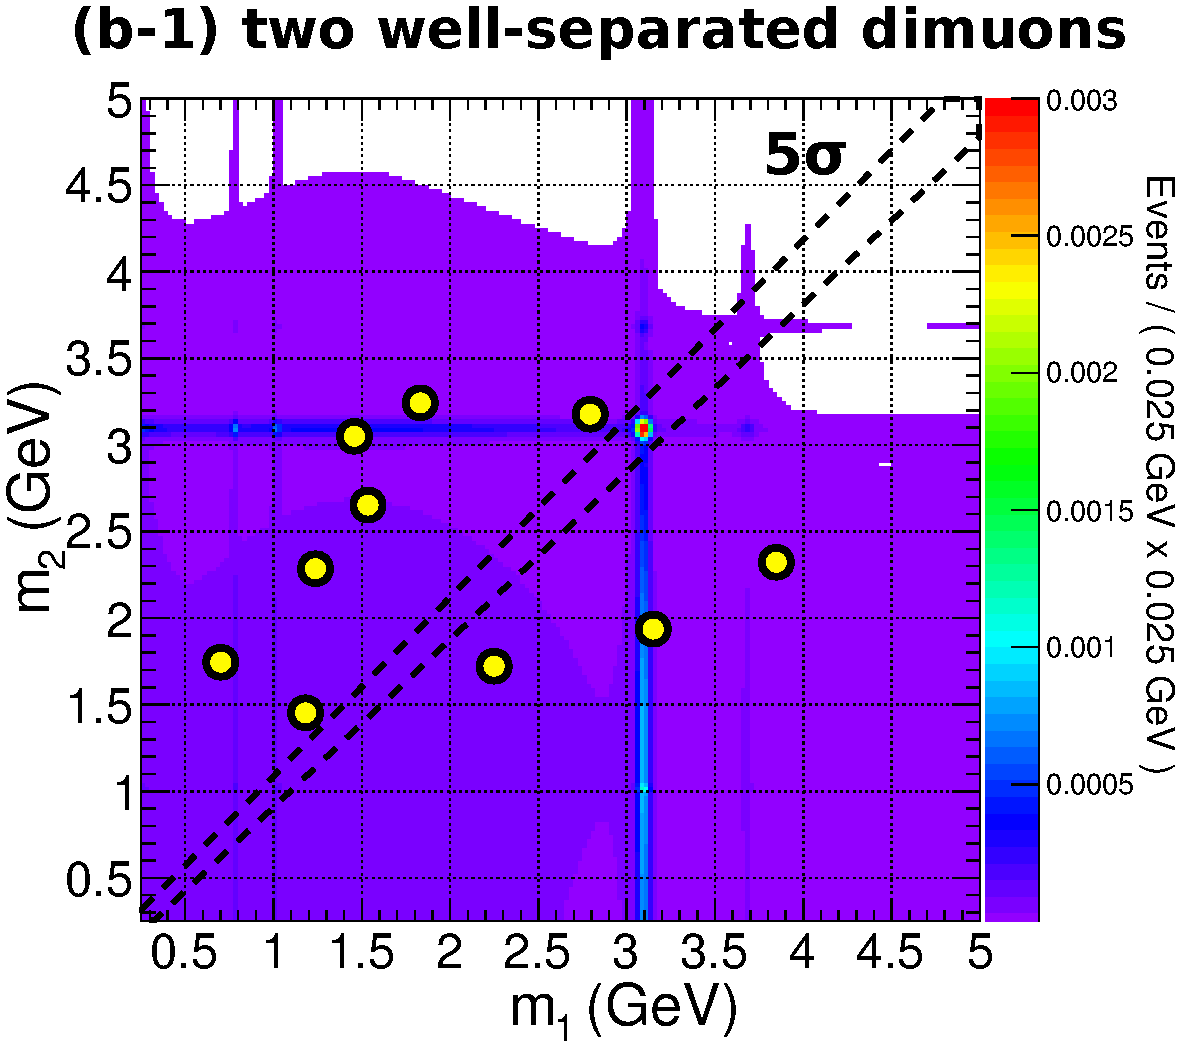
\includegraphics[width=\linewidth]{b1_2dpdf.pdf}
\end{columns}
\end{frame}

\begin{frame}
\vspace{0.75 cm}
\begin{center}
\textcolor{darkblue}{\large Event displays of double-dimuons (which have unequal masses)}
\end{center}

\begin{columns}
\column{0.63\linewidth}
\centering (a-2) two dimuons in one mu-jet

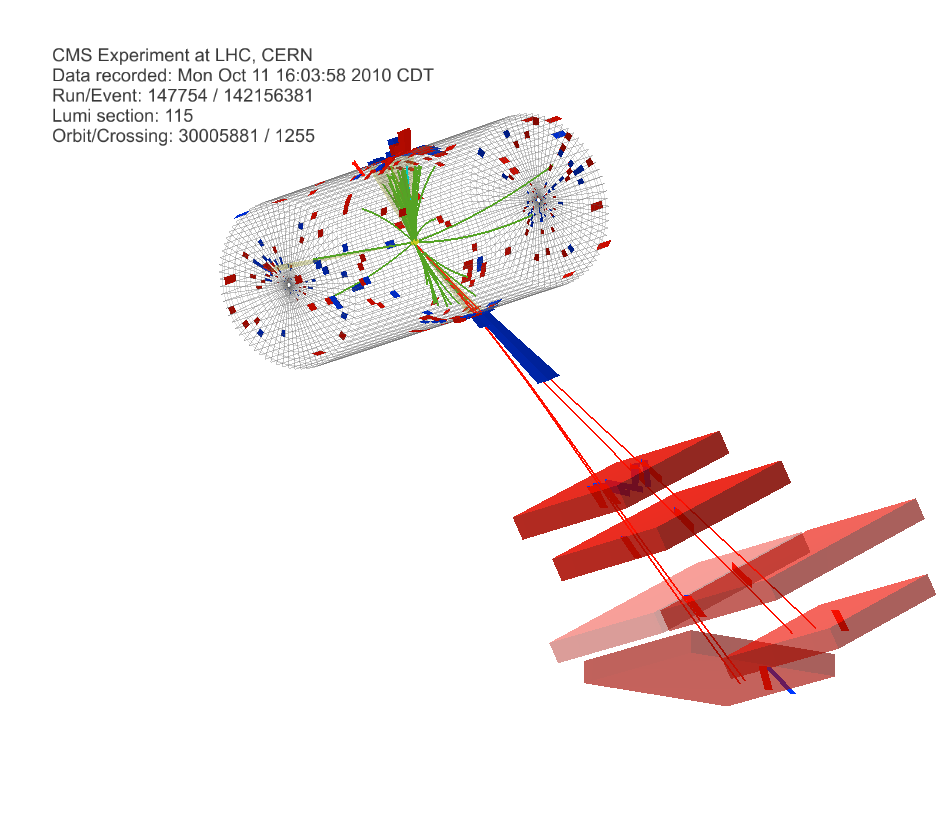
\includegraphics[width=\linewidth]{quadmu_control_eventdisplay.png}

\column{0.5\linewidth}
\centering (b-1) two well-separated dimuons

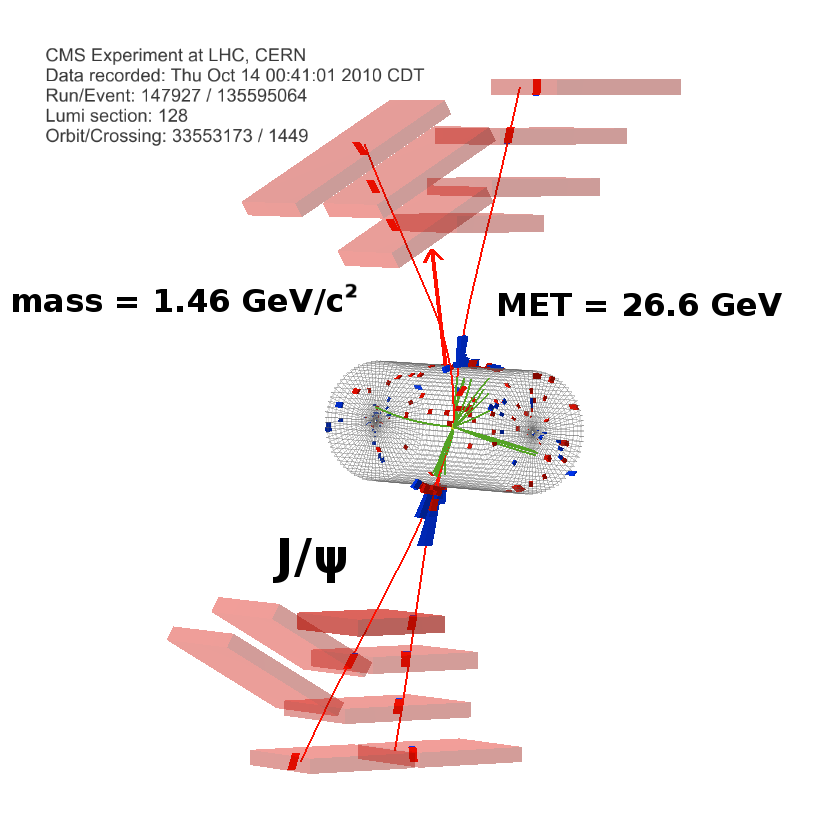
\includegraphics[width=\linewidth]{dimudimu_control_eventdisplay.png}
\end{columns}
\end{frame}

\begin{frame}
\frametitle{Limits}
\begin{itemize}
\item Limit-setting in RooFit/RooStats using the MCMC method
\item Luminosity, efficiency, and background shape systematics folded
  in (to be described later)
\item Set limits on $\sigma \times \mathcal{B} \times \alpha_\s{gen}$,
  where $\alpha_\s{gen}$ is the acceptance for a given model in a
  given signal region
\begin{itemize}
\item signature-based limit, applicable to future theories
\end{itemize}
\end{itemize}

\vfill
\begin{columns}
\column{0.33\linewidth}
\centering (a-1) one high-$p_T$ dimuon

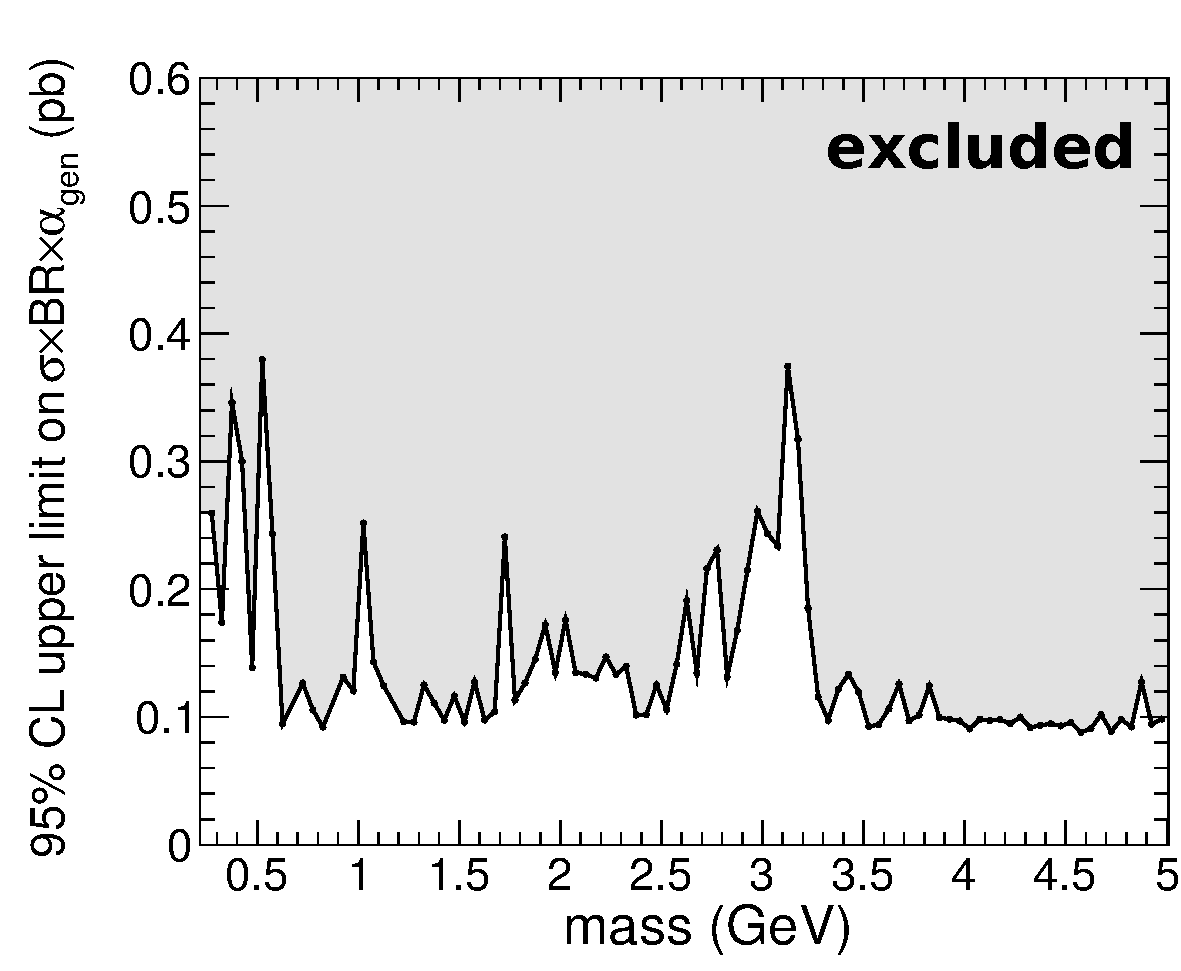
\includegraphics[width=\linewidth]{ul__sig_a1_n4.pdf}
\column{0.33\linewidth}
\centering (a-2) two dimuons in one mu-jet

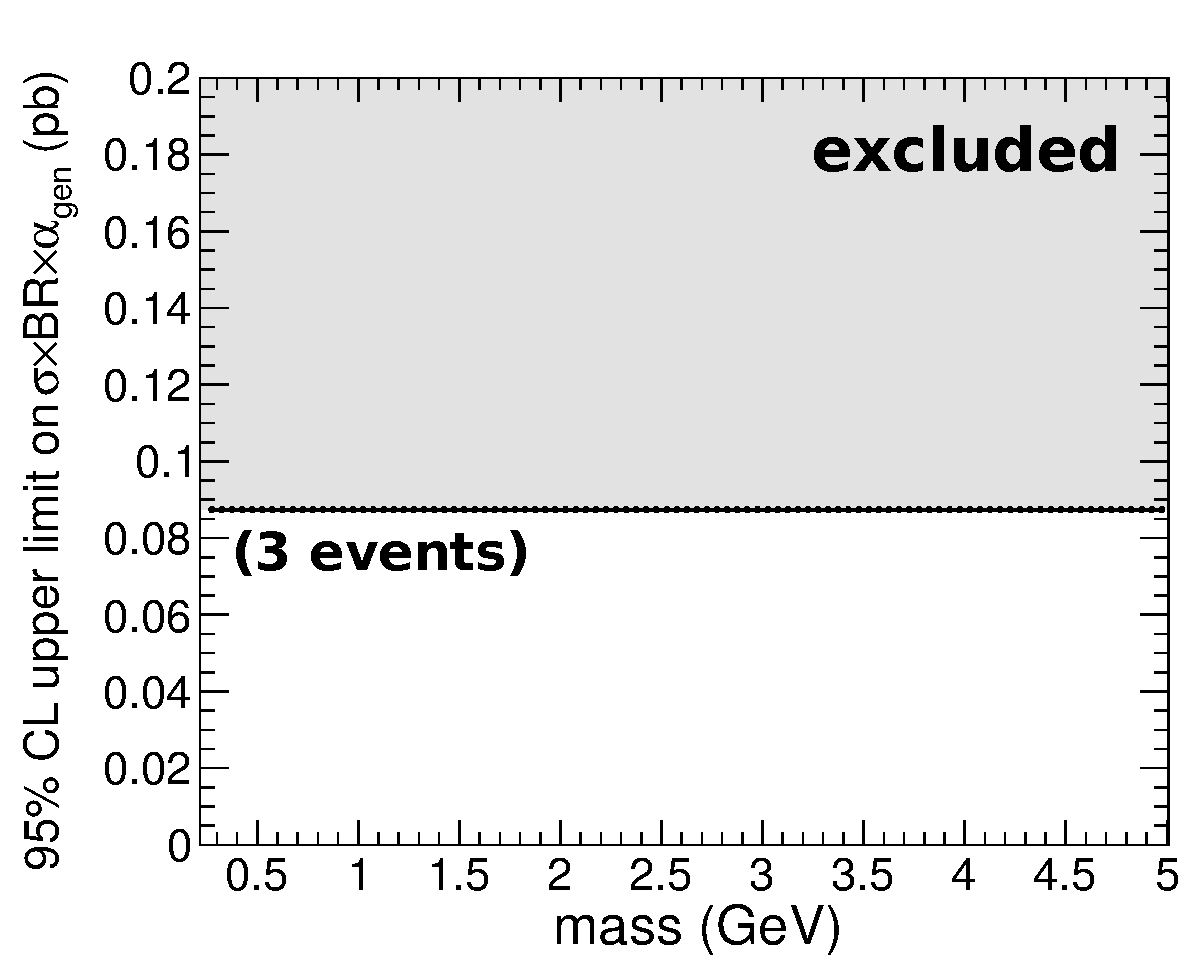
\includegraphics[width=\linewidth]{ul__sig_a2_n4.pdf}
\column{0.33\linewidth}
\centering (b-1) two well-separated dimuons

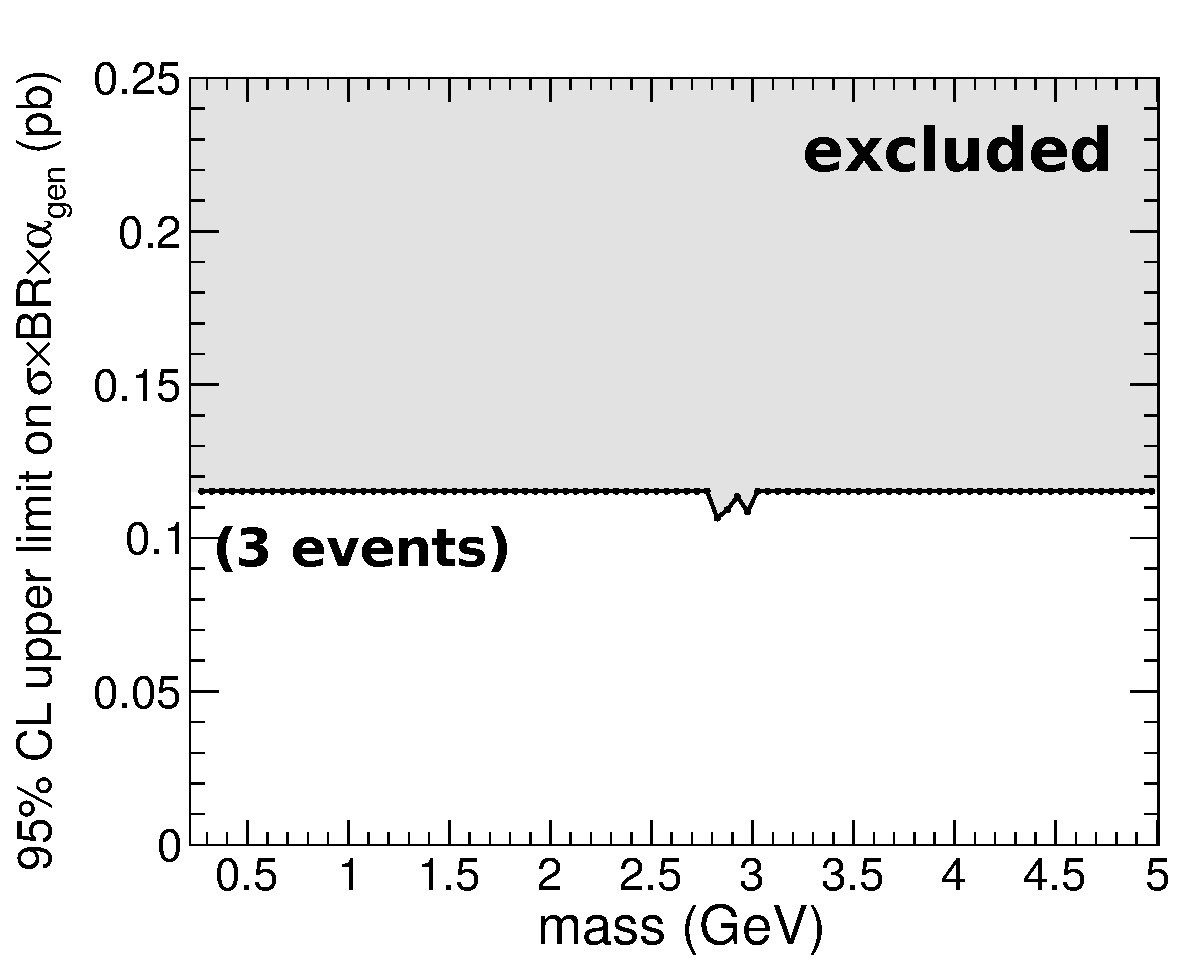
\includegraphics[width=\linewidth]{ul__sig_b1_n3.pdf}
\end{columns}

All other signal regions (3 or more dimuons per event) are also
excluded at the level of 0.1~pb, independent of $m_1$ mass $<$ 5~GeV/$c^2$
\end{frame}

\section*{Fit Shape Templates}
\begin{frame}

\vfill
\begin{center}
\Huge \textcolor{blue}{Fit Shape Templates}
\end{center}

\vfill
\end{frame}

\begin{frame}
\frametitle{Signal shape (the easy part)}

\begin{itemize}
\item Since the hidden sector couples weakly to the Standard Model,
  the $m_1$ resonance width must be dominated by detector resolution
\item We have four Standard Model resonances in our
  background-enriched dataset (single dimuon, $p_T < 80$~GeV/$c$)
\end{itemize}

\mbox{ }\hfill 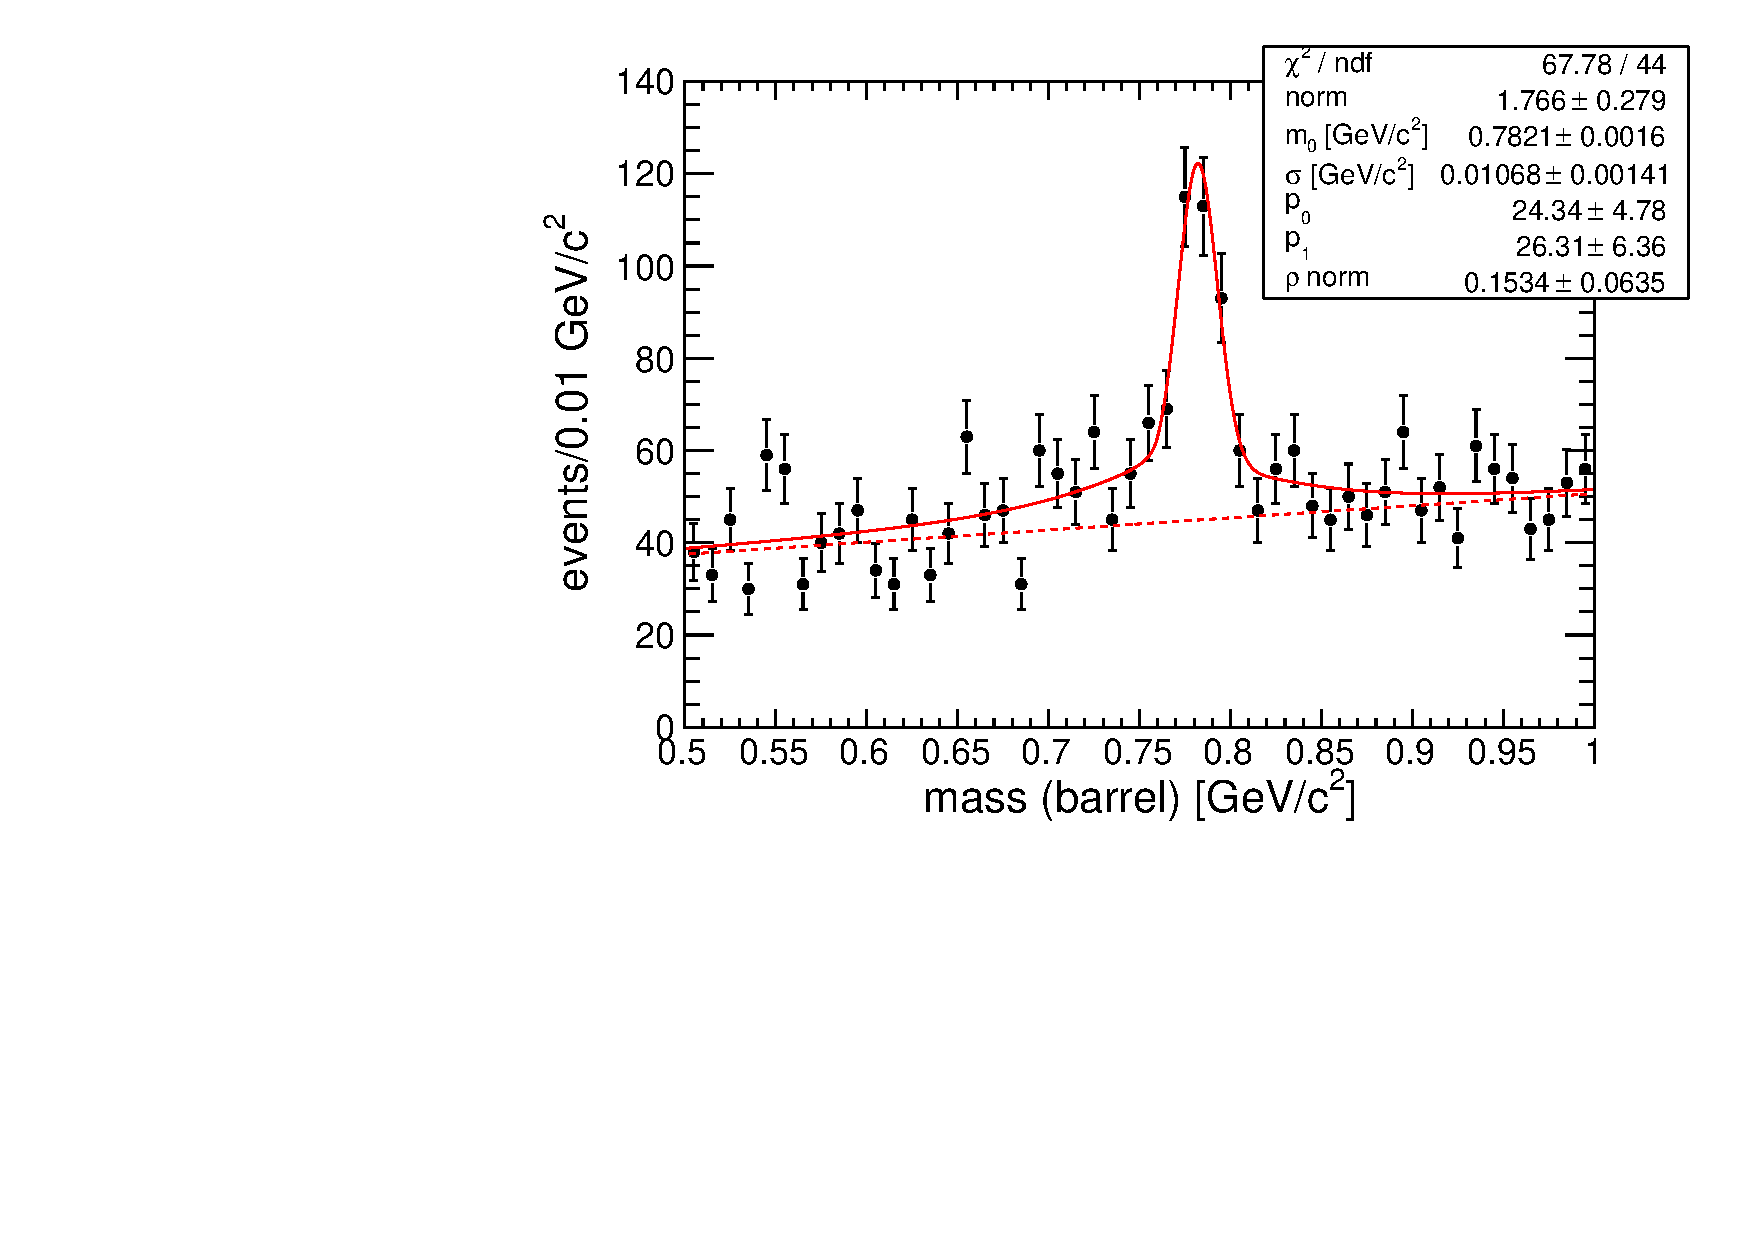
\includegraphics[width=0.4\linewidth]{respeak_omega_barrel.pdf} \hfill
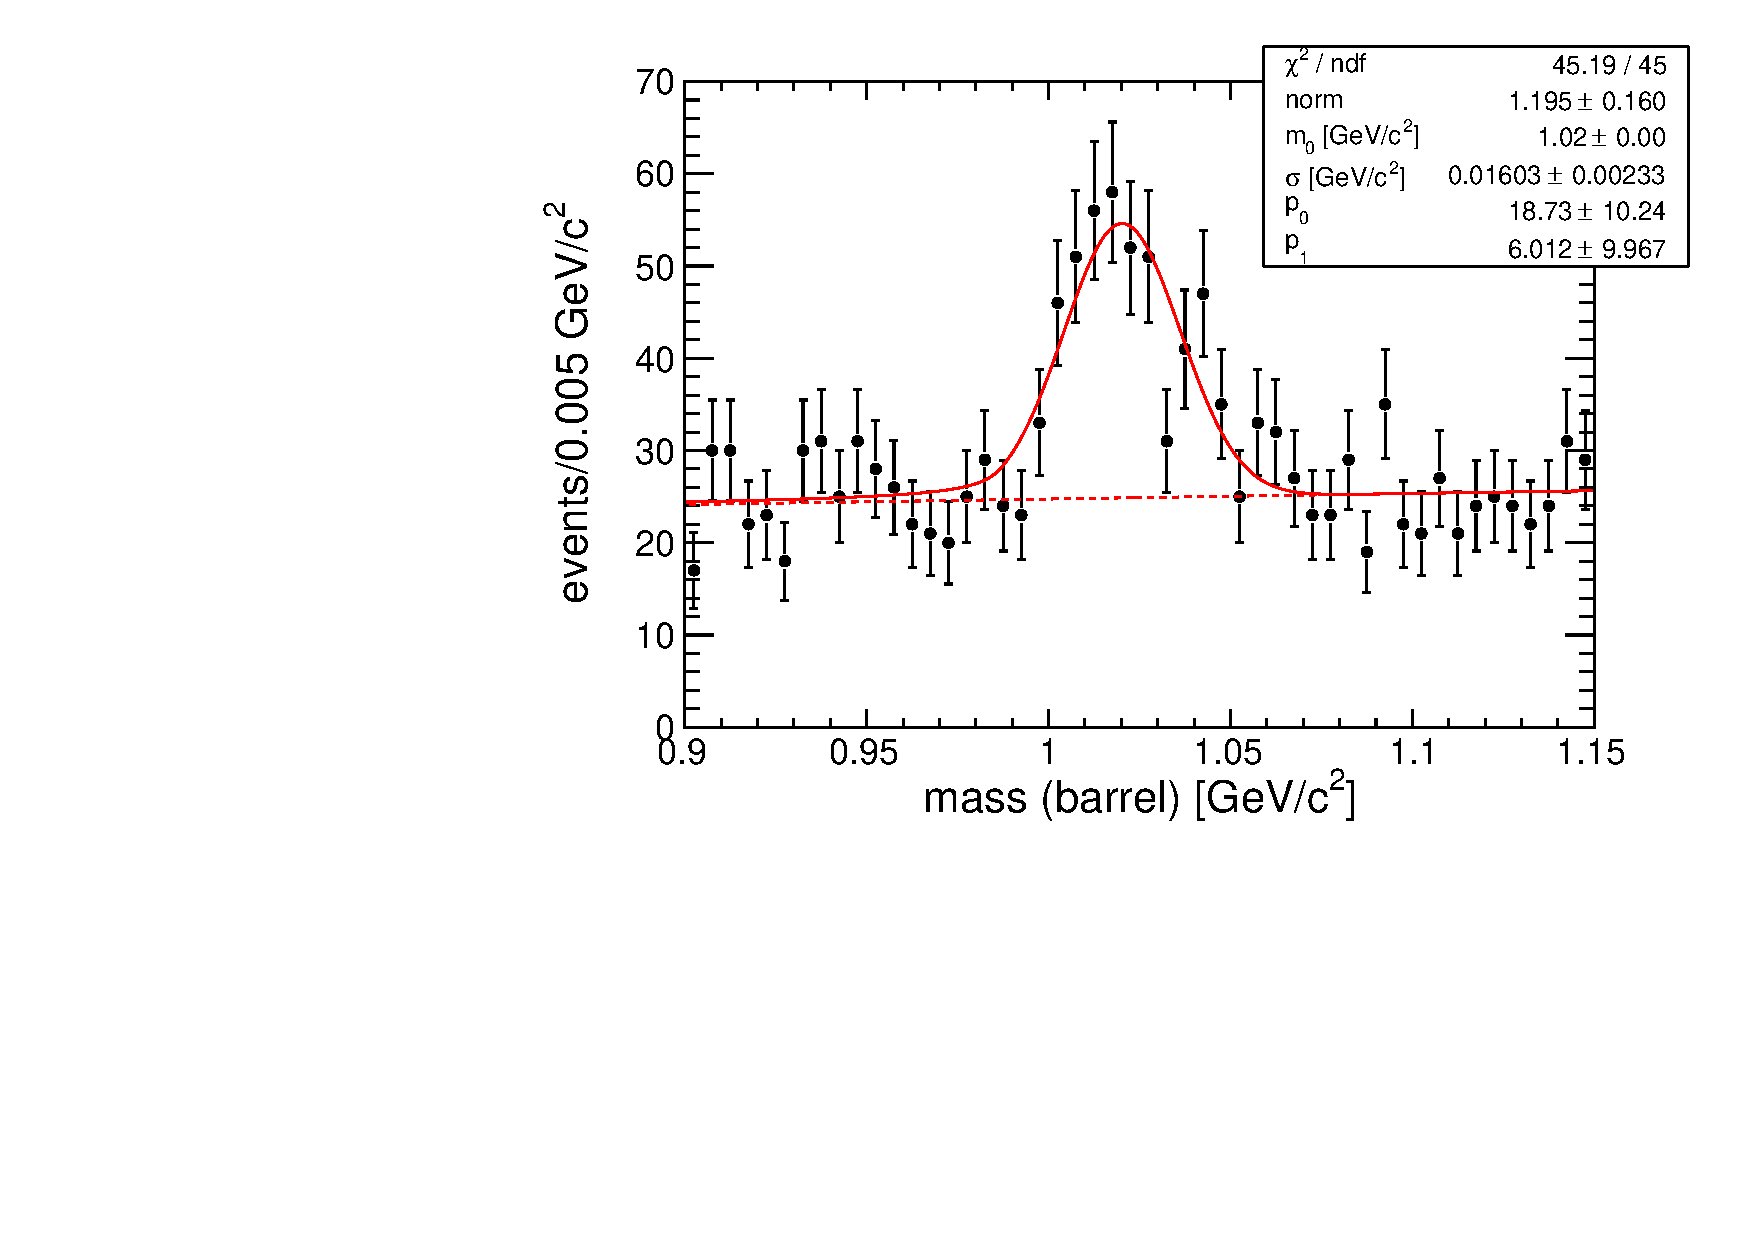
\includegraphics[width=0.4\linewidth]{respeak_phi_barrel.pdf} \hfill \mbox{ } \\
\mbox{ }\hfill 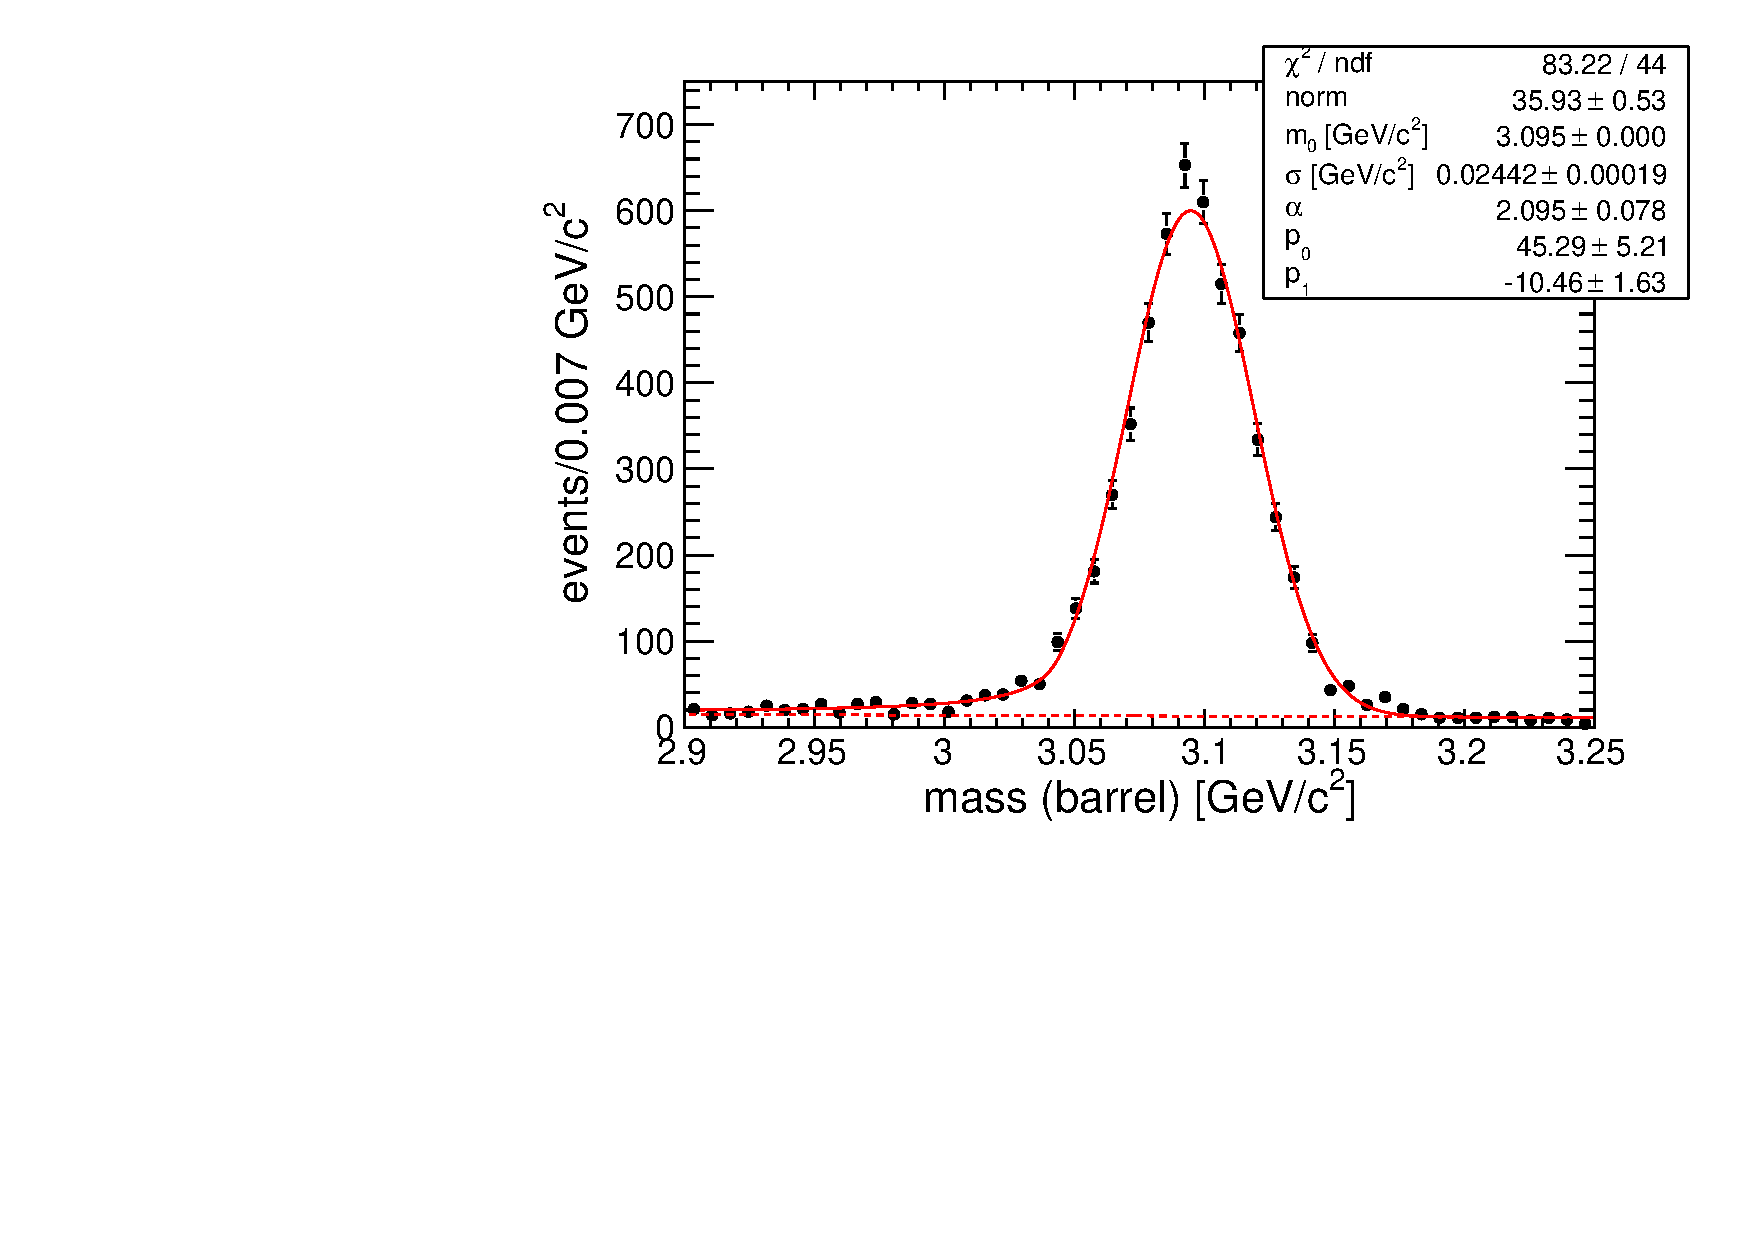
\includegraphics[width=0.4\linewidth]{respeak_jpsi_barrel.pdf} \hfill
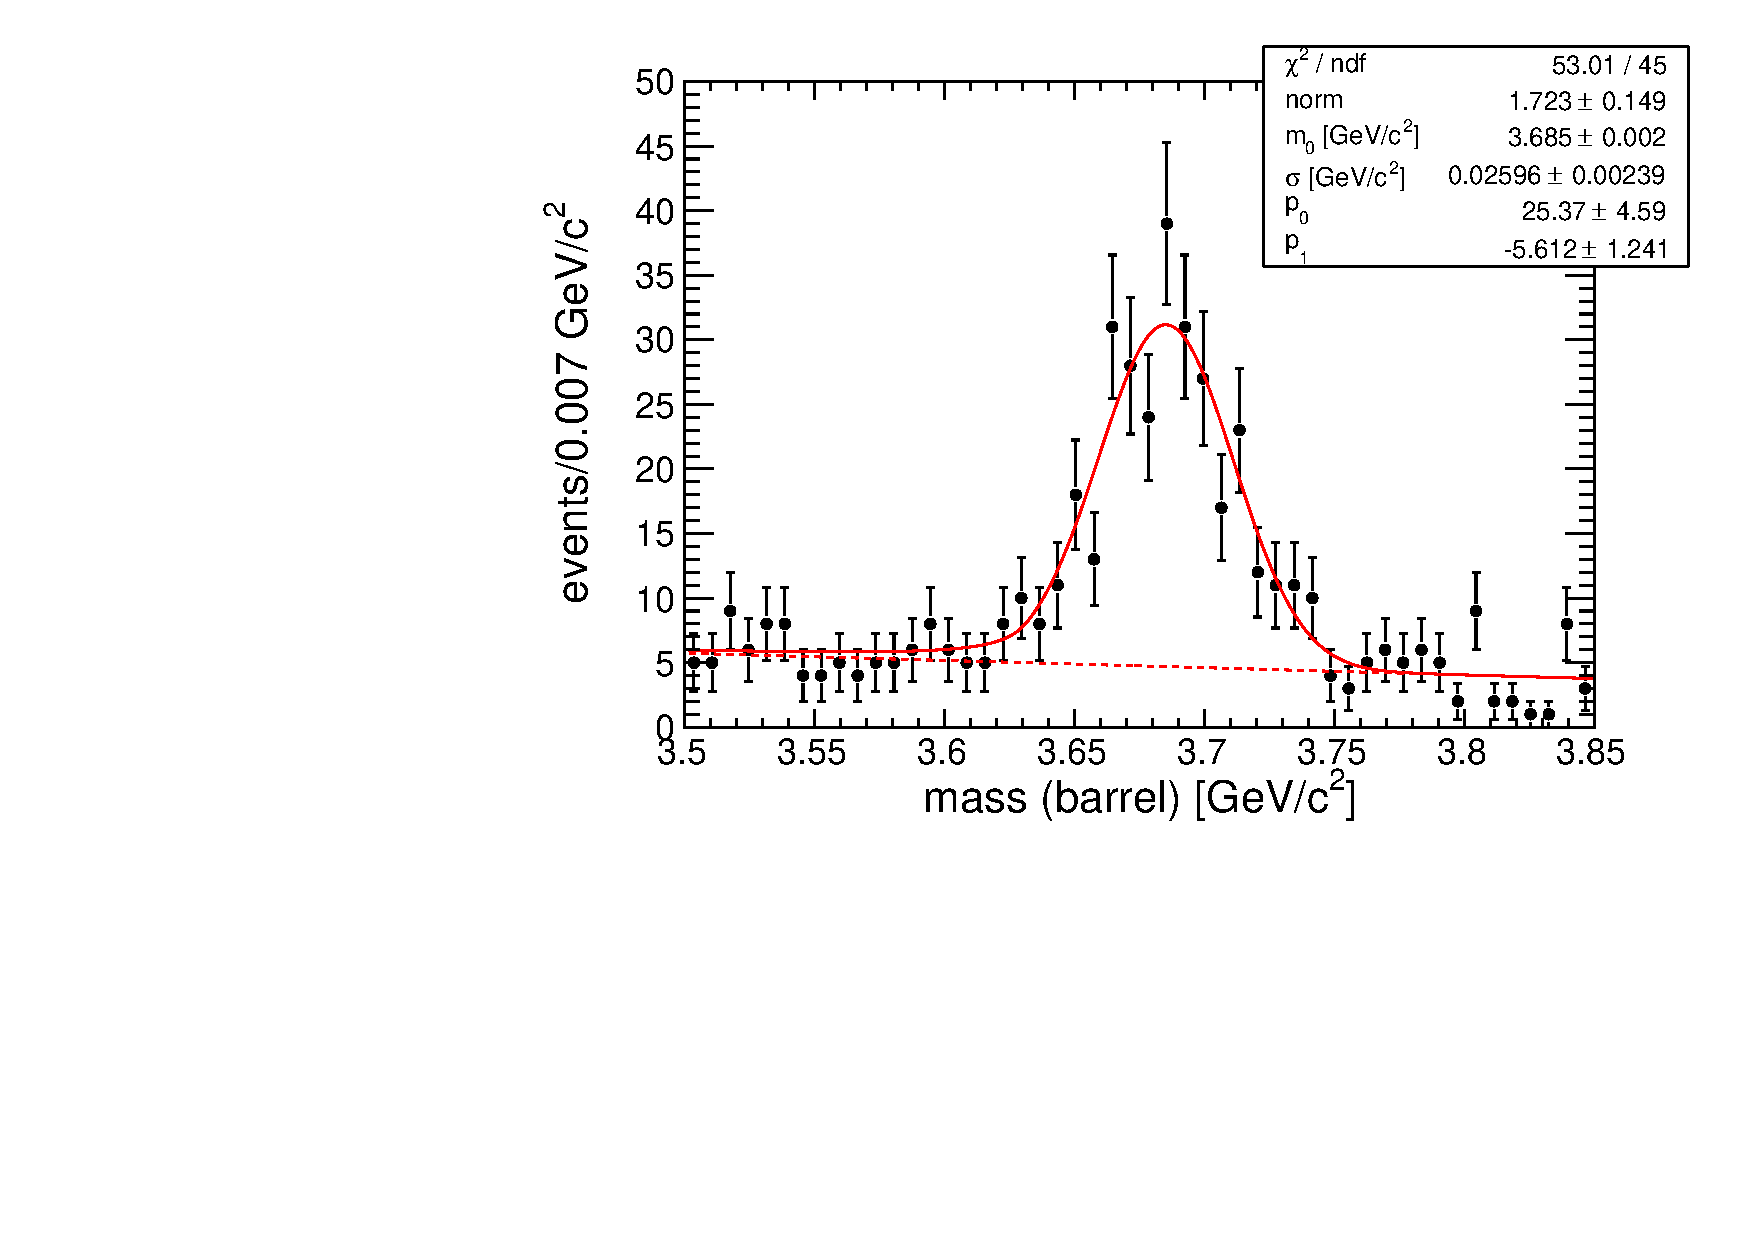
\includegraphics[width=0.4\linewidth]{respeak_psiprime_barrel.pdf} \hfill \mbox{ } \\
\end{frame}

\begin{frame}
\frametitle{Signal shape (the easy part)}

\vfill
\begin{columns}
\column{0.5\linewidth}
\centering Barrel ($|\eta| < 0.9$)

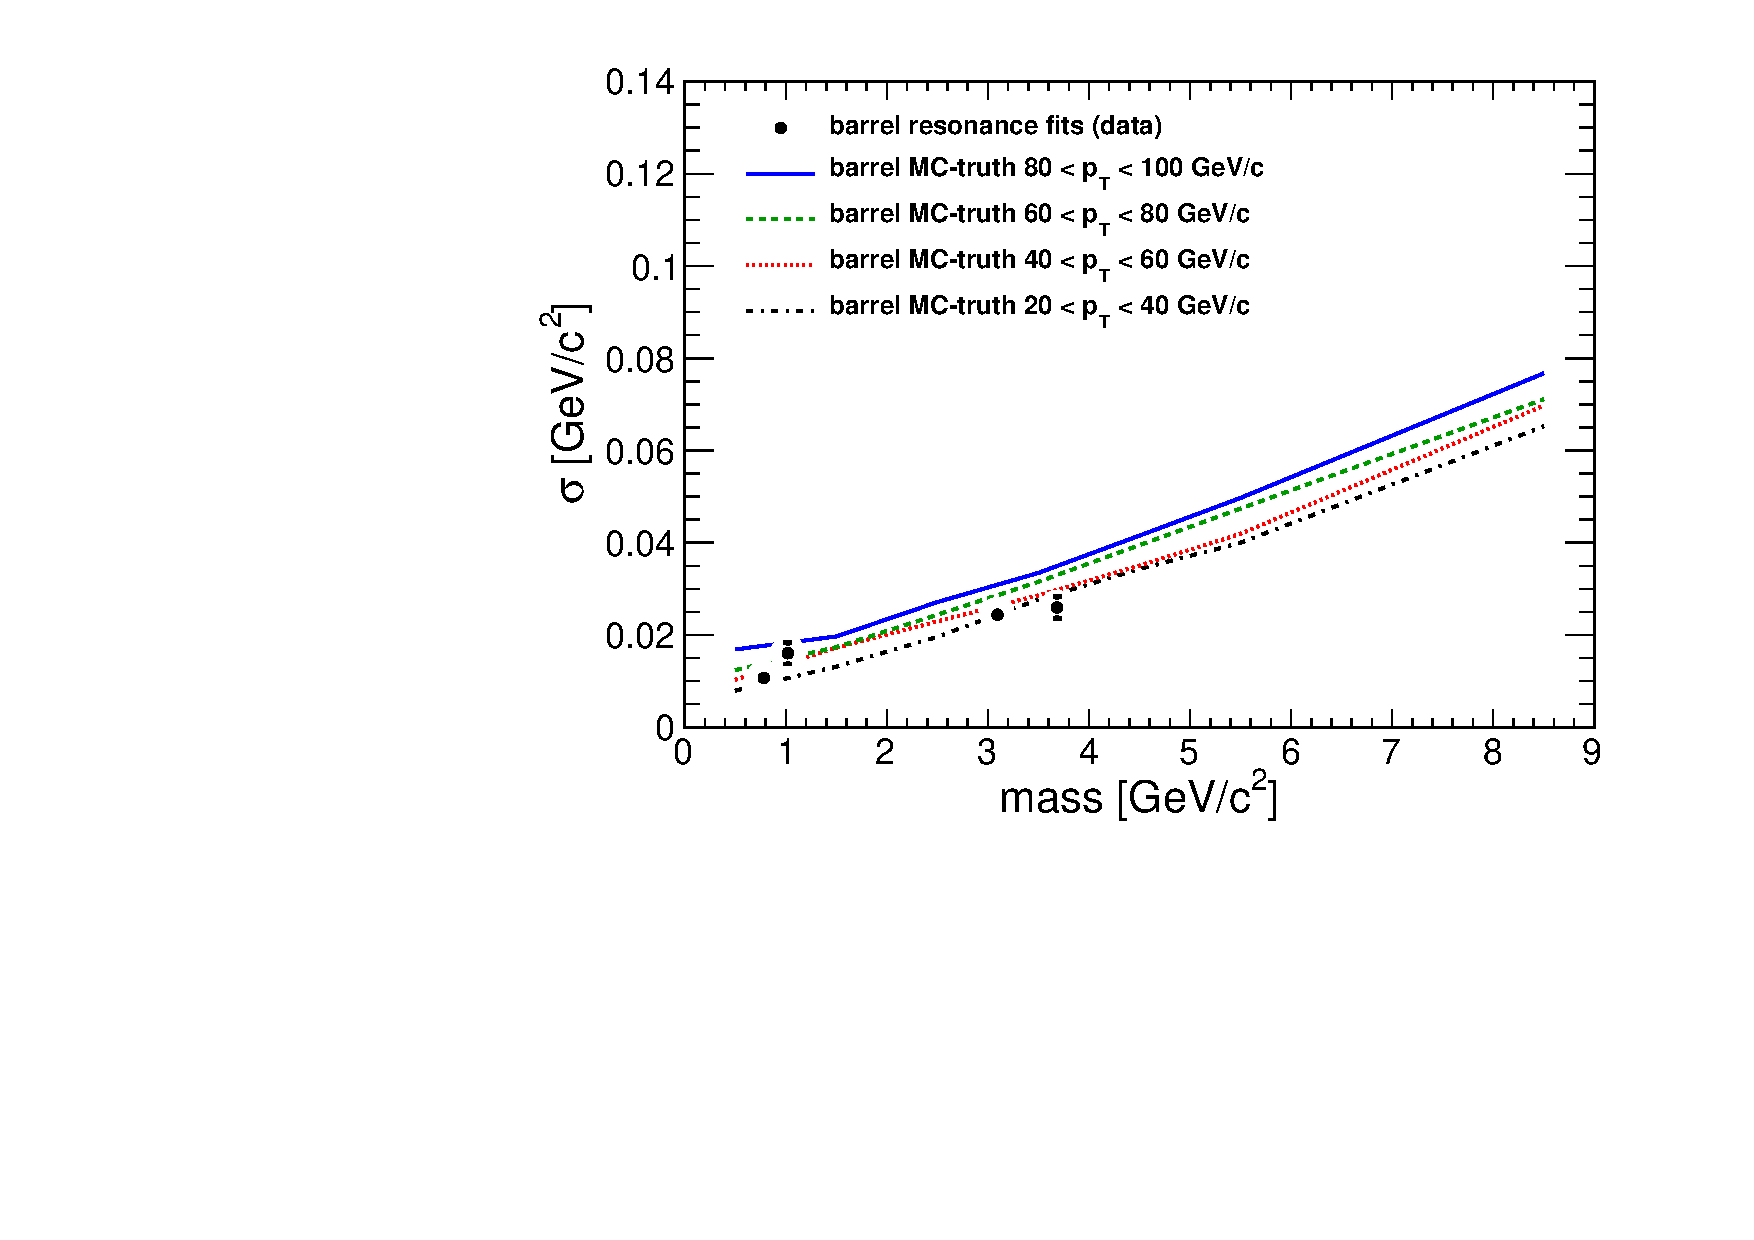
\includegraphics[width=\linewidth]{resolution_barrel.pdf}

\column{0.5\linewidth}
\centering Endcap ($|\eta| > 0.9$)

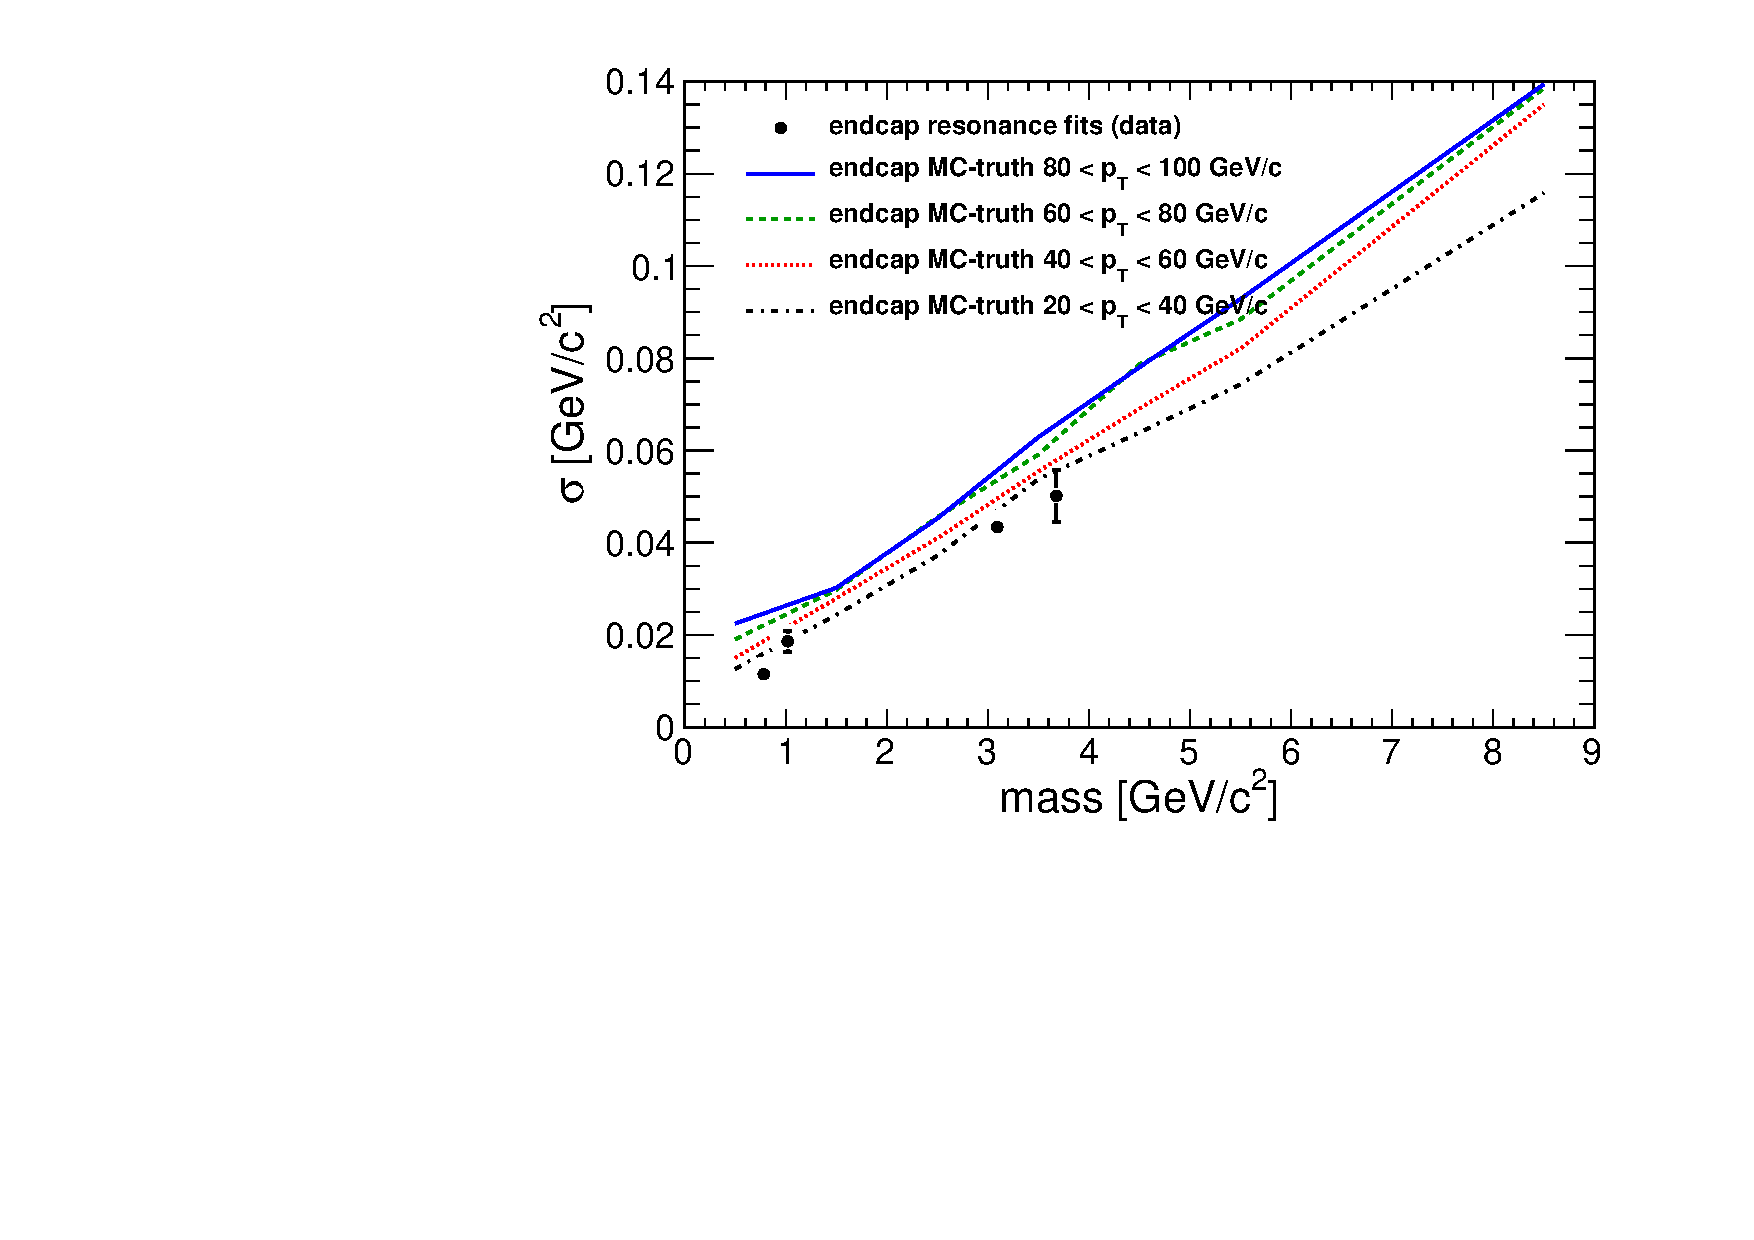
\includegraphics[width=\linewidth]{resolution_endcap.pdf}
\end{columns}

\begin{itemize}
\item Different resolution in the barrel and endcap
\item Filled in resolution vs.\ mass and $p_T$ with MC pair-gun
\item Data agree well with the minimum-$p_T$ curve
\item Modeled in final fit as double-Gaussian (barrel and endcap) with
  a Crystal Ball radiative tail, $p_T$ variation is a systematic uncertainty
\end{itemize}
\end{frame}

\begin{frame}
\frametitle{Background shape}

\begin{itemize}
\item Different physics sources contribute to each signal region, so
  the background shape templates must be individually constructed

\hfill 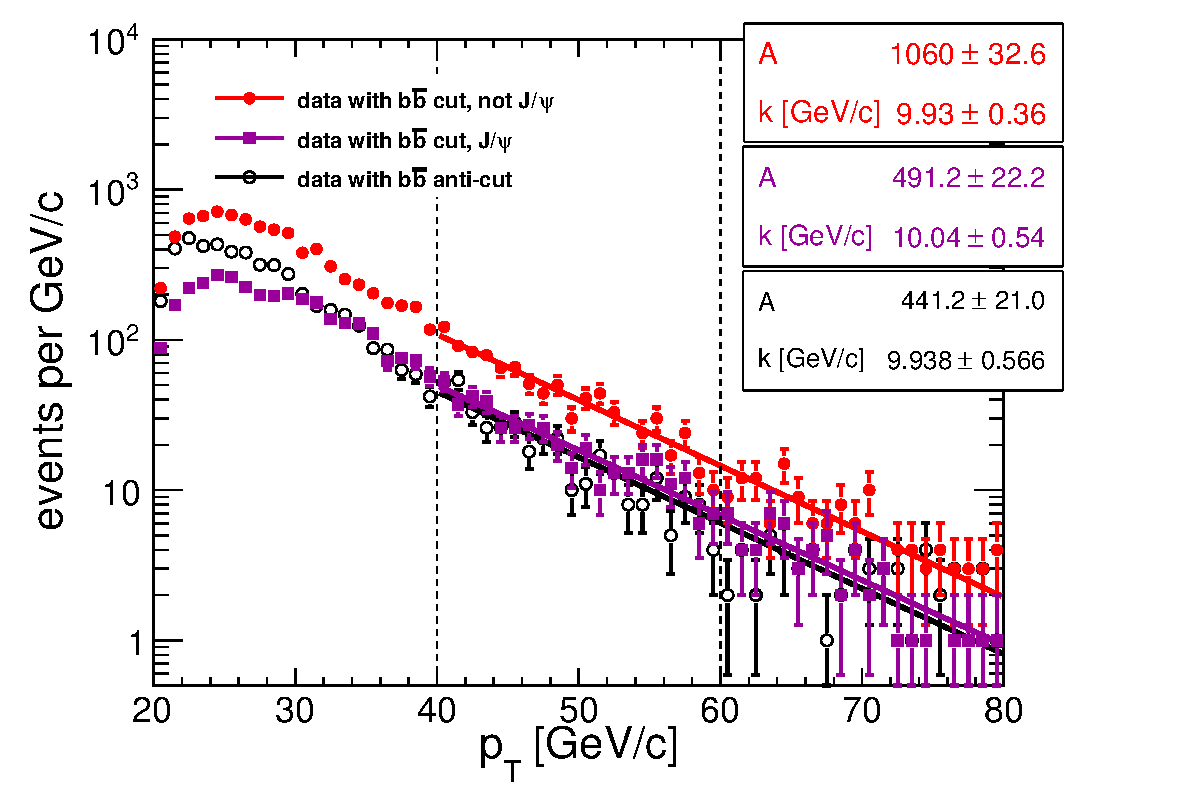
\includegraphics[width=0.50\linewidth]{support_bbbarcut_limits.pdf}

\vspace{-3.5 cm}
\item For (a-1): prompt \& isolated, \\ \textcolor{red}{$b\bar{b}$-like,} \textcolor{violet}{and $J/\psi$} components \\ all scale as {\scriptsize $\exp(-p_T/10\mbox{ GeV})$} \\ above 40~GeV/$c$

\item Derive shape from high-statistics \\ low-$p_T$ data, test in medium-$p_T$, \\ and use in high-$p_T$ signal search
\end{itemize}

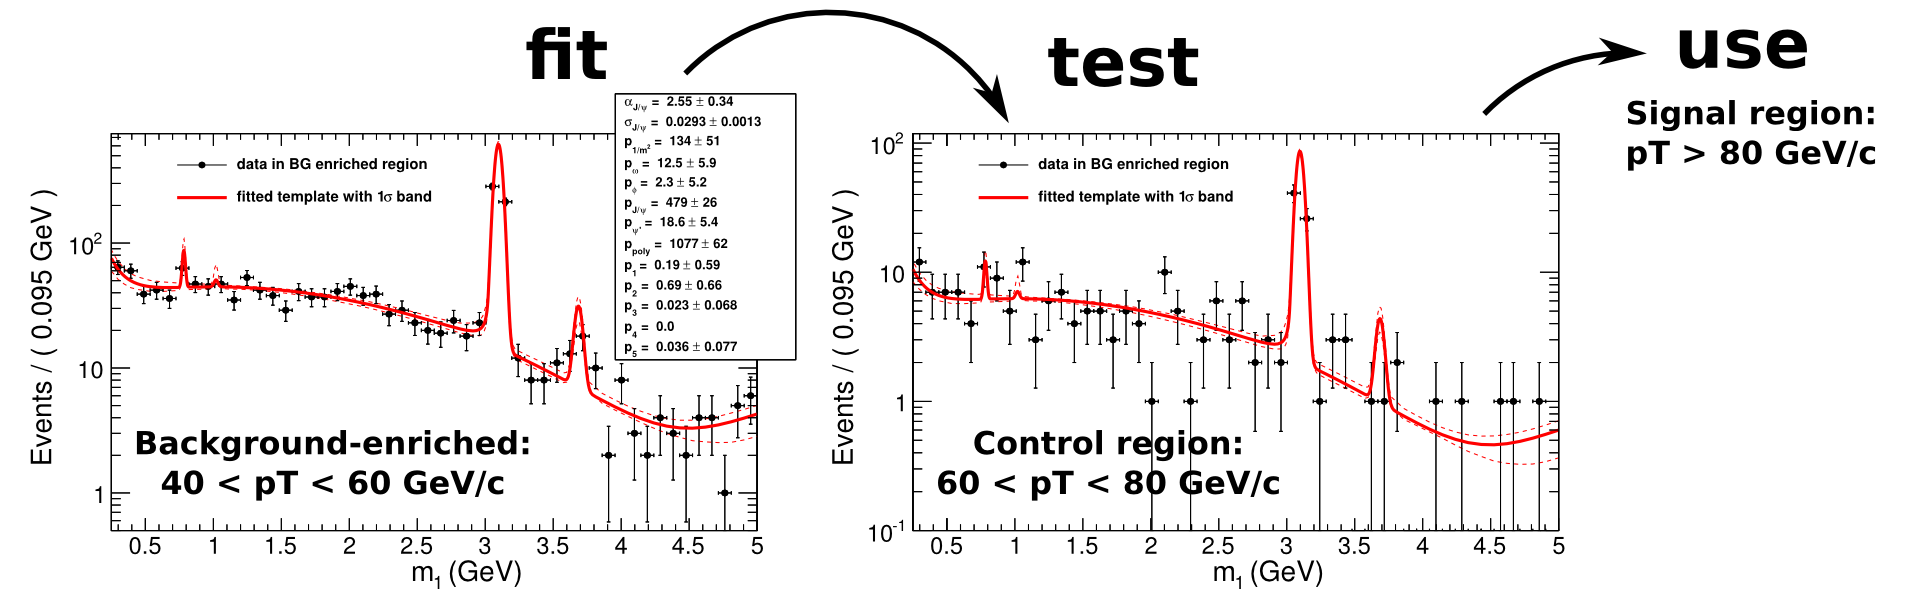
\includegraphics[width=\linewidth]{background_shape_a1.png}
\end{frame}

\begin{frame}
\frametitle{Background shape}

\hfill 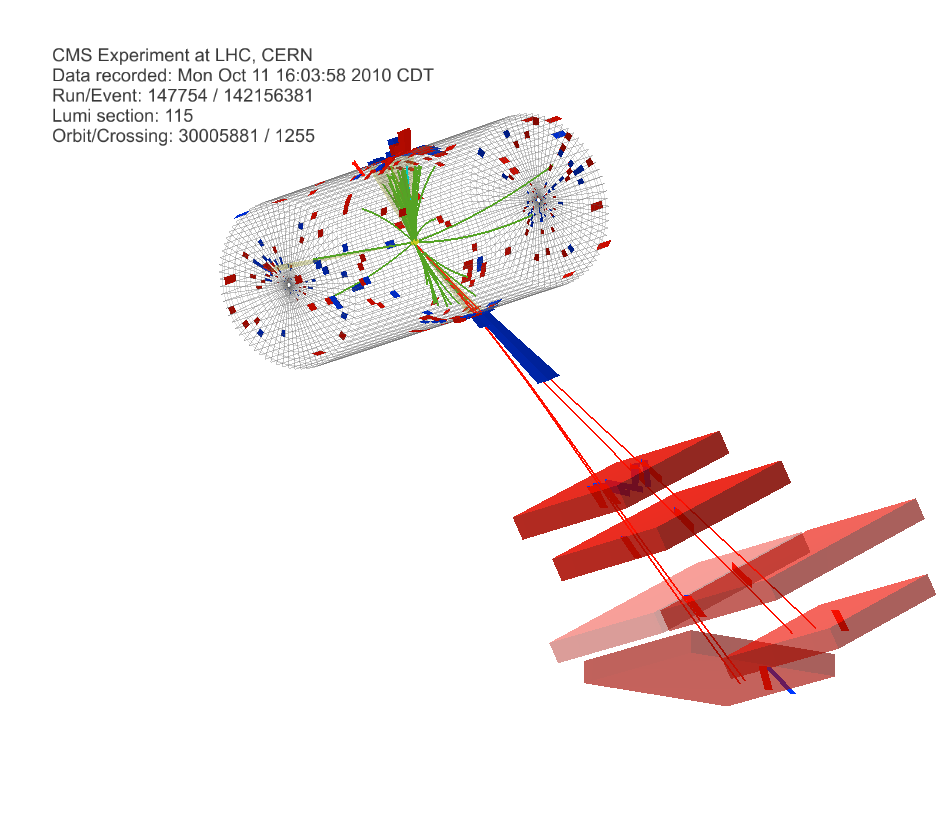
\includegraphics[height=3 cm]{quadmu_control_eventdisplay.png}

\vspace{-3 cm}
\begin{itemize}
\item Region (a-2): 4 muons in one mu-jet

\item Dominant Standard Model backgrounds: \\ decays-in-flight and misreconstruction (fakes)

\item Simulate fake muons by putting non-muon \\ tracks into mu-jets:
\end{itemize}

\vspace{-0.4 cm}
\renewcommand{\arraystretch}{1.3}
\begin{center}
\begin{tabular}{c c c}
Background-enriched & Control & Signal Region \\\hline
2 muons, 2 tracks & 3 muons, 1 track & 4 muons
\end{tabular}
\end{center}

\vspace{-0.2 cm}
\begin{itemize}
\item Plots of control region with template shape overlaid:
\end{itemize}

\vspace{-0.2 cm}
\mbox{ } \hfill 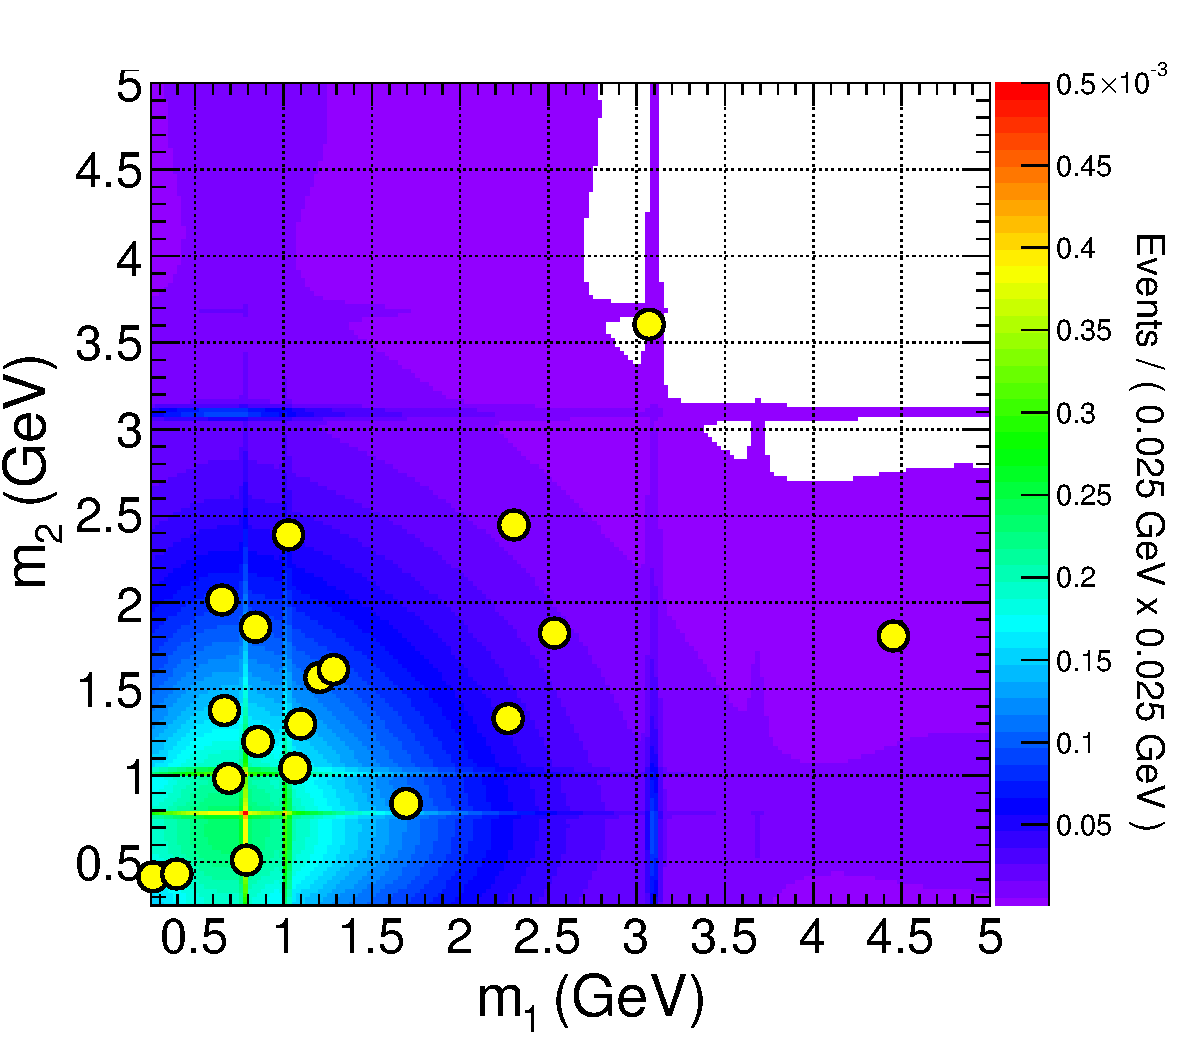
\includegraphics[height=3.5 cm]{a2_control.pdf} \hfill
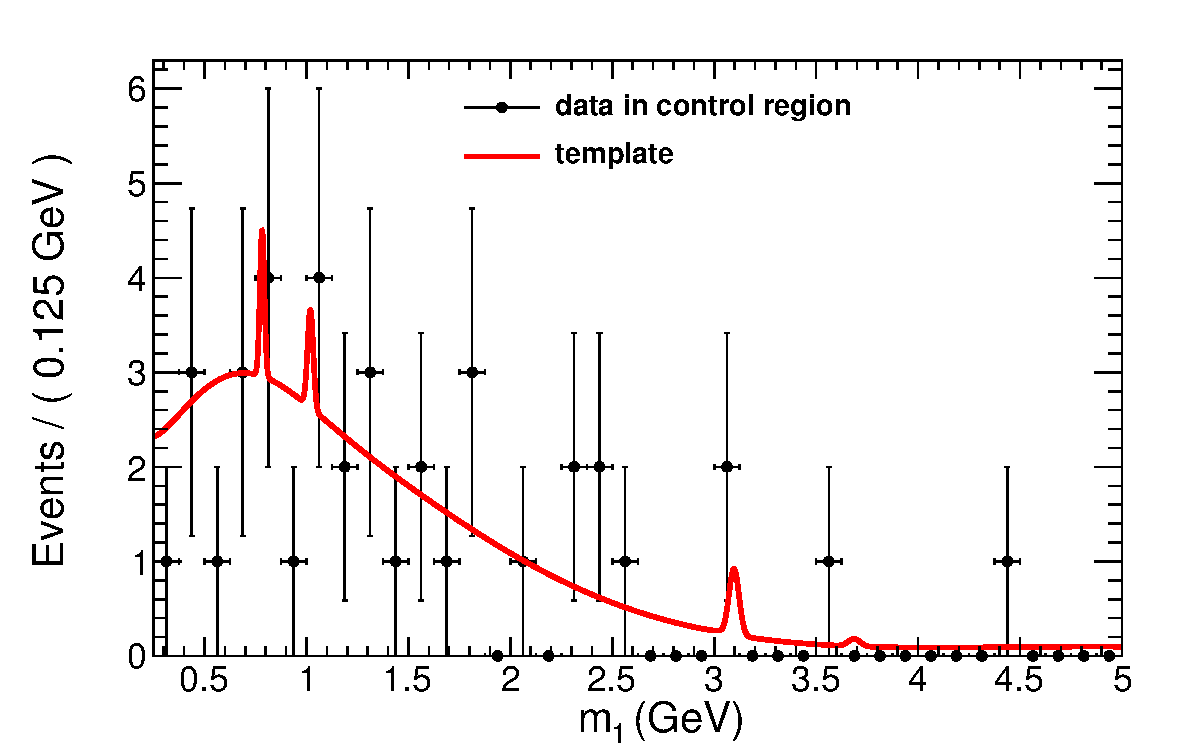
\includegraphics[height=3.5 cm]{template_control__bkg_model_a2__m_1.pdf} \hfill \mbox{ }
\end{frame}

\begin{frame}
\frametitle{Background shape}

\hfill 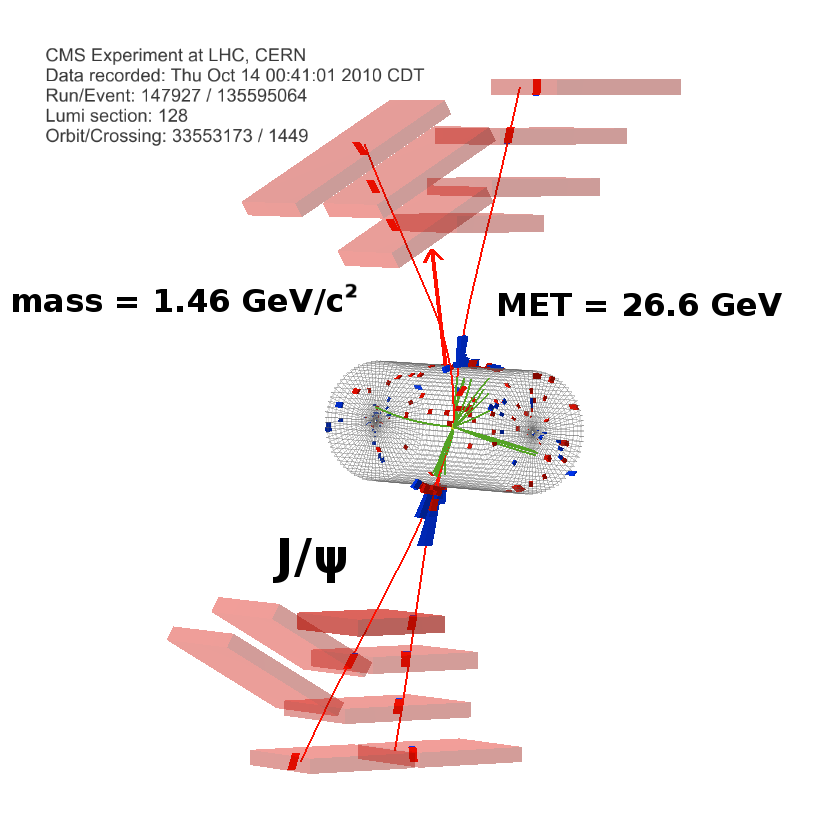
\includegraphics[height=3.5 cm]{dimudimu_control_eventdisplay.png}

\vspace{-3.5 cm}
\begin{itemize}
\item Region (b-1): 2 mu-jets with 2 muons each
\item Dominant Standard Model backgrounds: \\ $b\bar{b}$ with both
  $b$-quarks producing $\mu\mu X$ by \\ double-semileptonic decay,
  resonances, etc.
\item Assume that each $b$-quark decays independently \\ and construct
  2-D distribution from Cartesian \\ product of 1-D $b\to\mu\mu X$ distributions

\item Background-enriched: selected dimuons (left); \\ control region: off-diagonal part of signal (right; already seen)
\end{itemize}

\mbox{ } \hfill 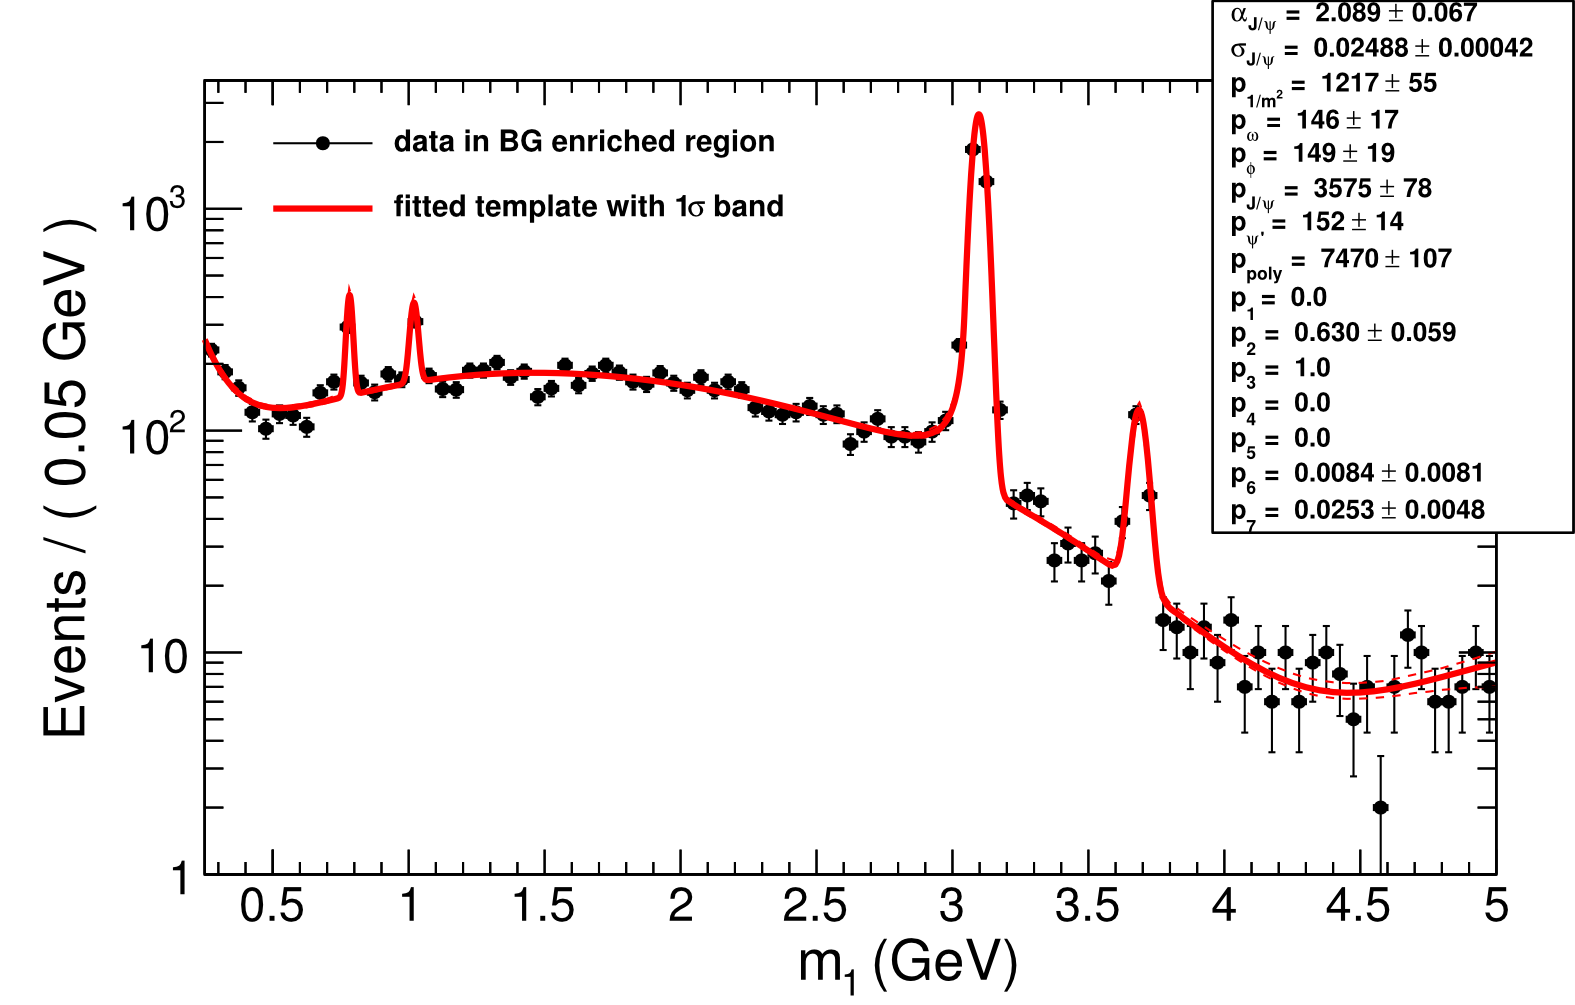
\includegraphics[height=3 cm]{template__bg_sh_b1t__m_1_log.png} \hfill 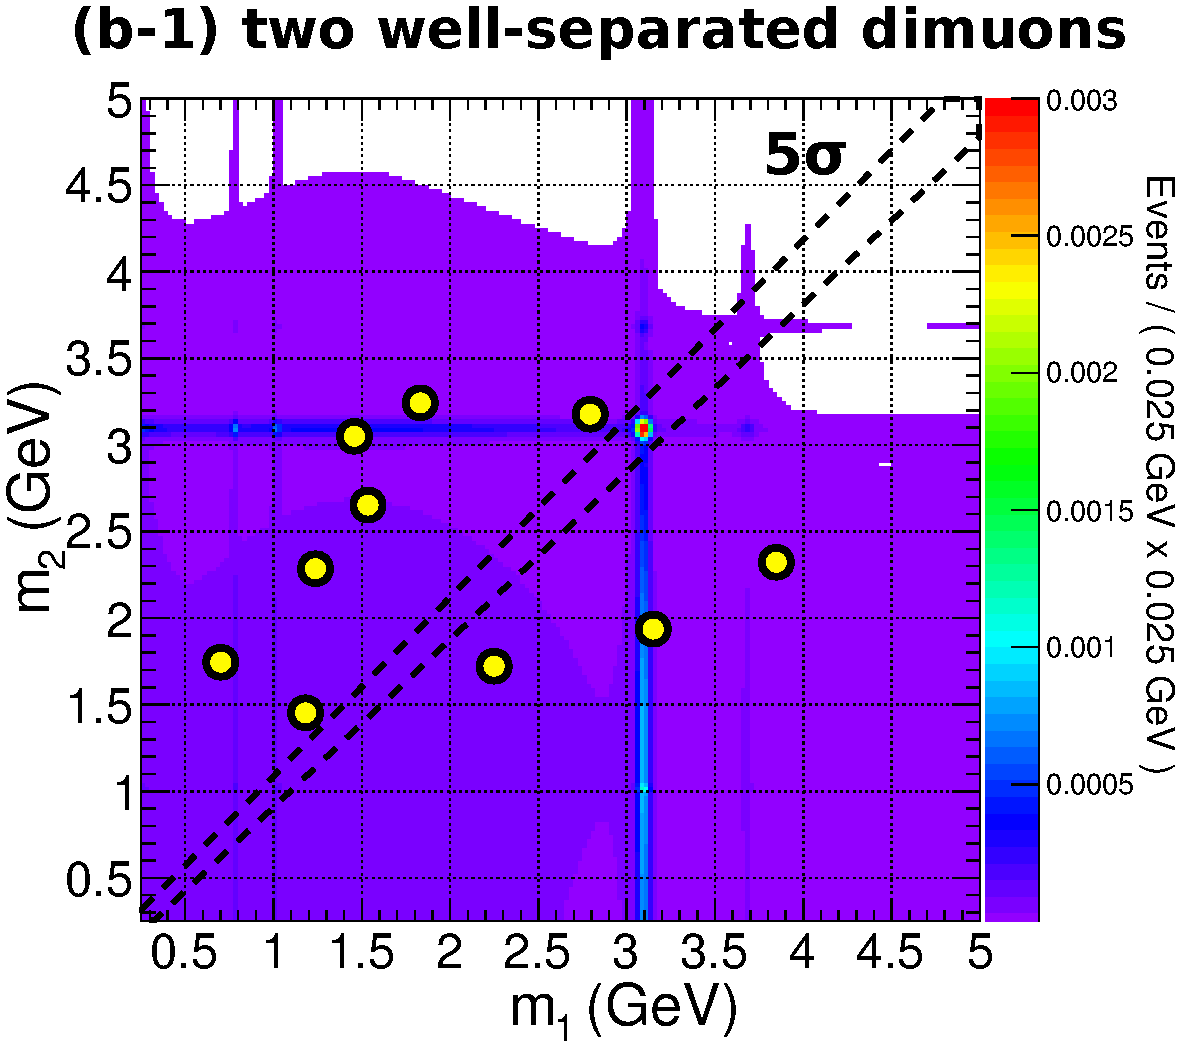
\includegraphics[height=3 cm]{b1_2dpdf.pdf} \hfill \mbox{ }
\end{frame}

\section*{Detector Issues and Acceptance}
\begin{frame}

\vfill
\begin{center}
\Huge \textcolor{blue}{Detector Issues and Acceptance}
\end{center}

\vfill
\end{frame}

\begin{frame}
\frametitle{Trigger efficiency}

\begin{itemize}
\item Some triggers' efficiencies depend strongly on whether the muon
  trajectories cross in the muon system
\begin{itemize}
\item this is a problem for a model-independent study because
  different models have different fractions of muon crossing
\item parameterizing it would make the results too complicated
\end{itemize}

\item Trigger efficiency vs.\ $\eta$ for crossing and \textcolor{red}{non-crossing} muons:
\end{itemize}

\begin{columns}
\column{0.33\linewidth}
\centering single-muon (Mu15)

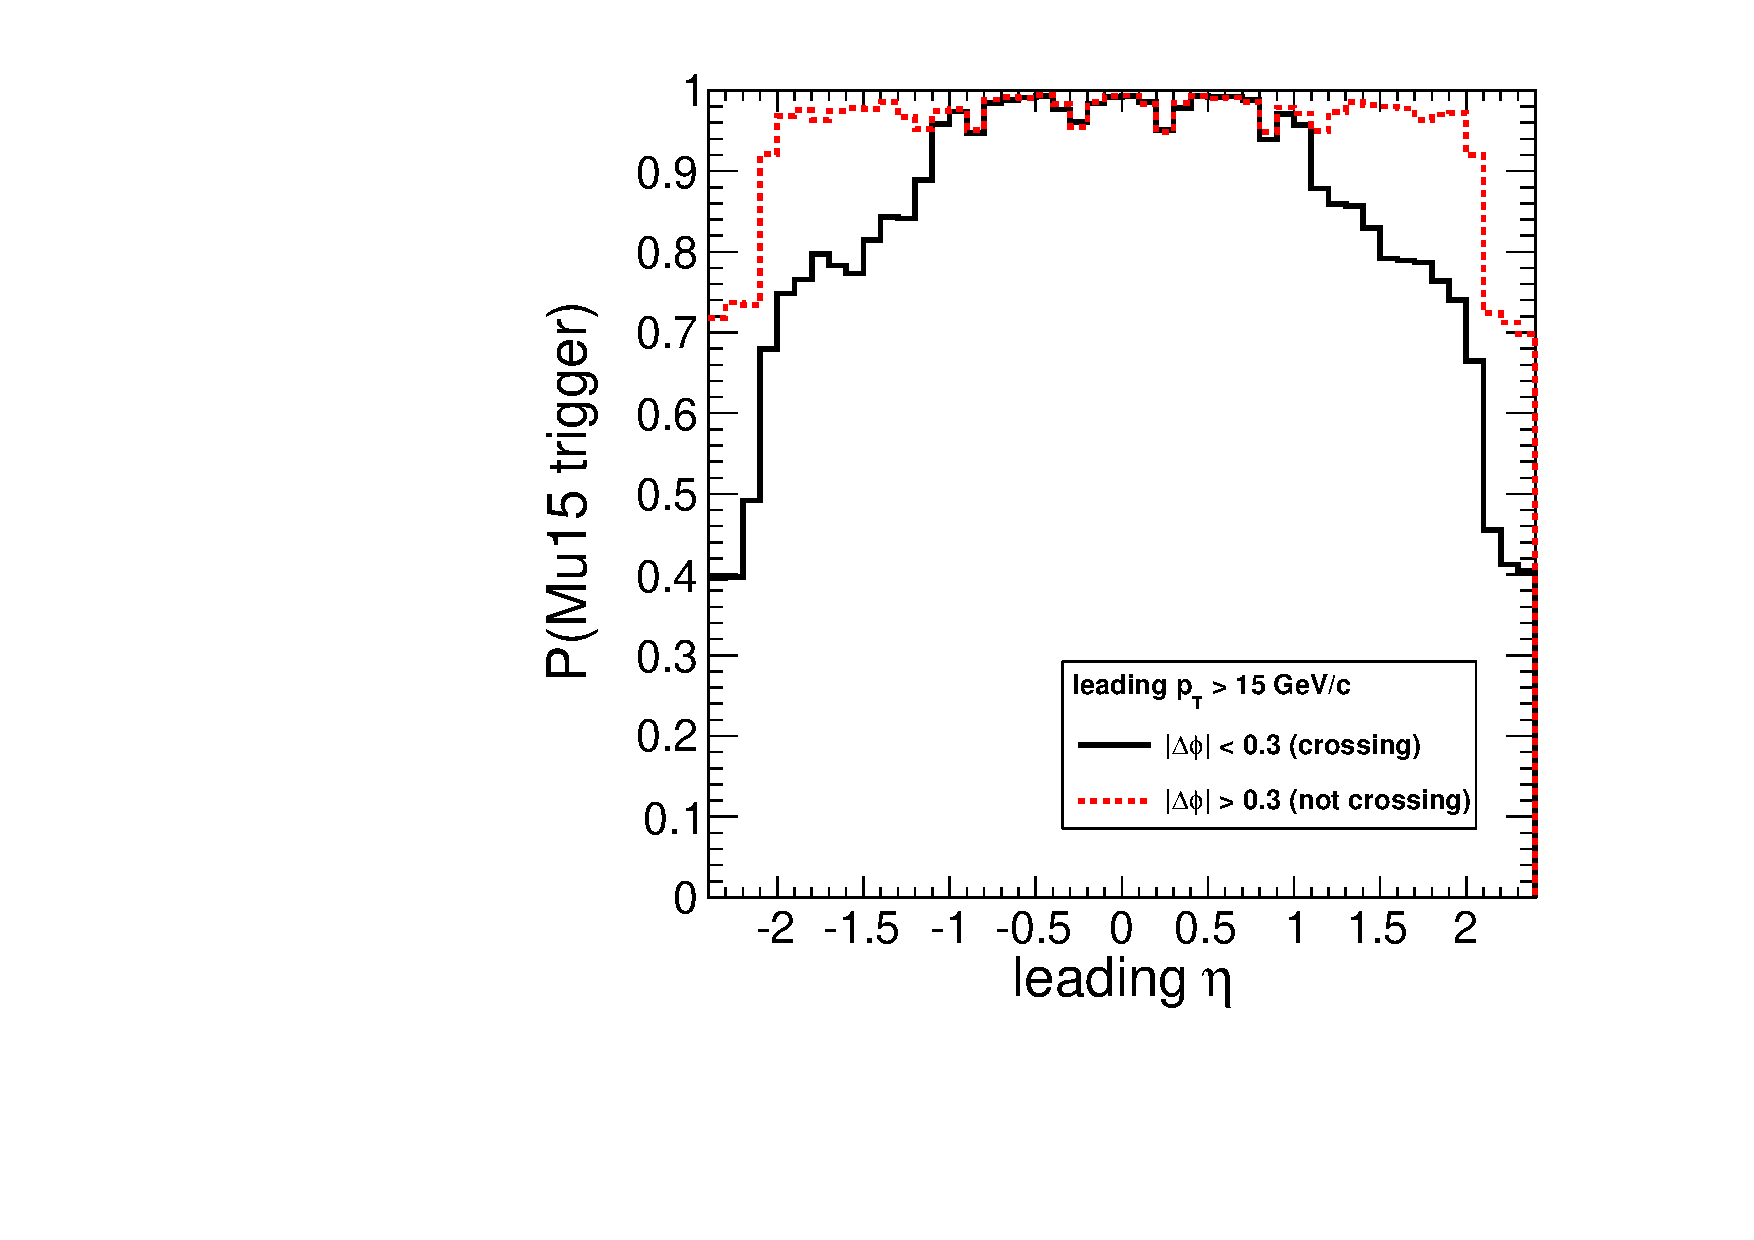
\includegraphics[width=\linewidth]{eta_mass5cut_triggerMu15_nosuppressedzero.pdf}

\column{0.33\linewidth}
\centering isolated (IsoMu9)

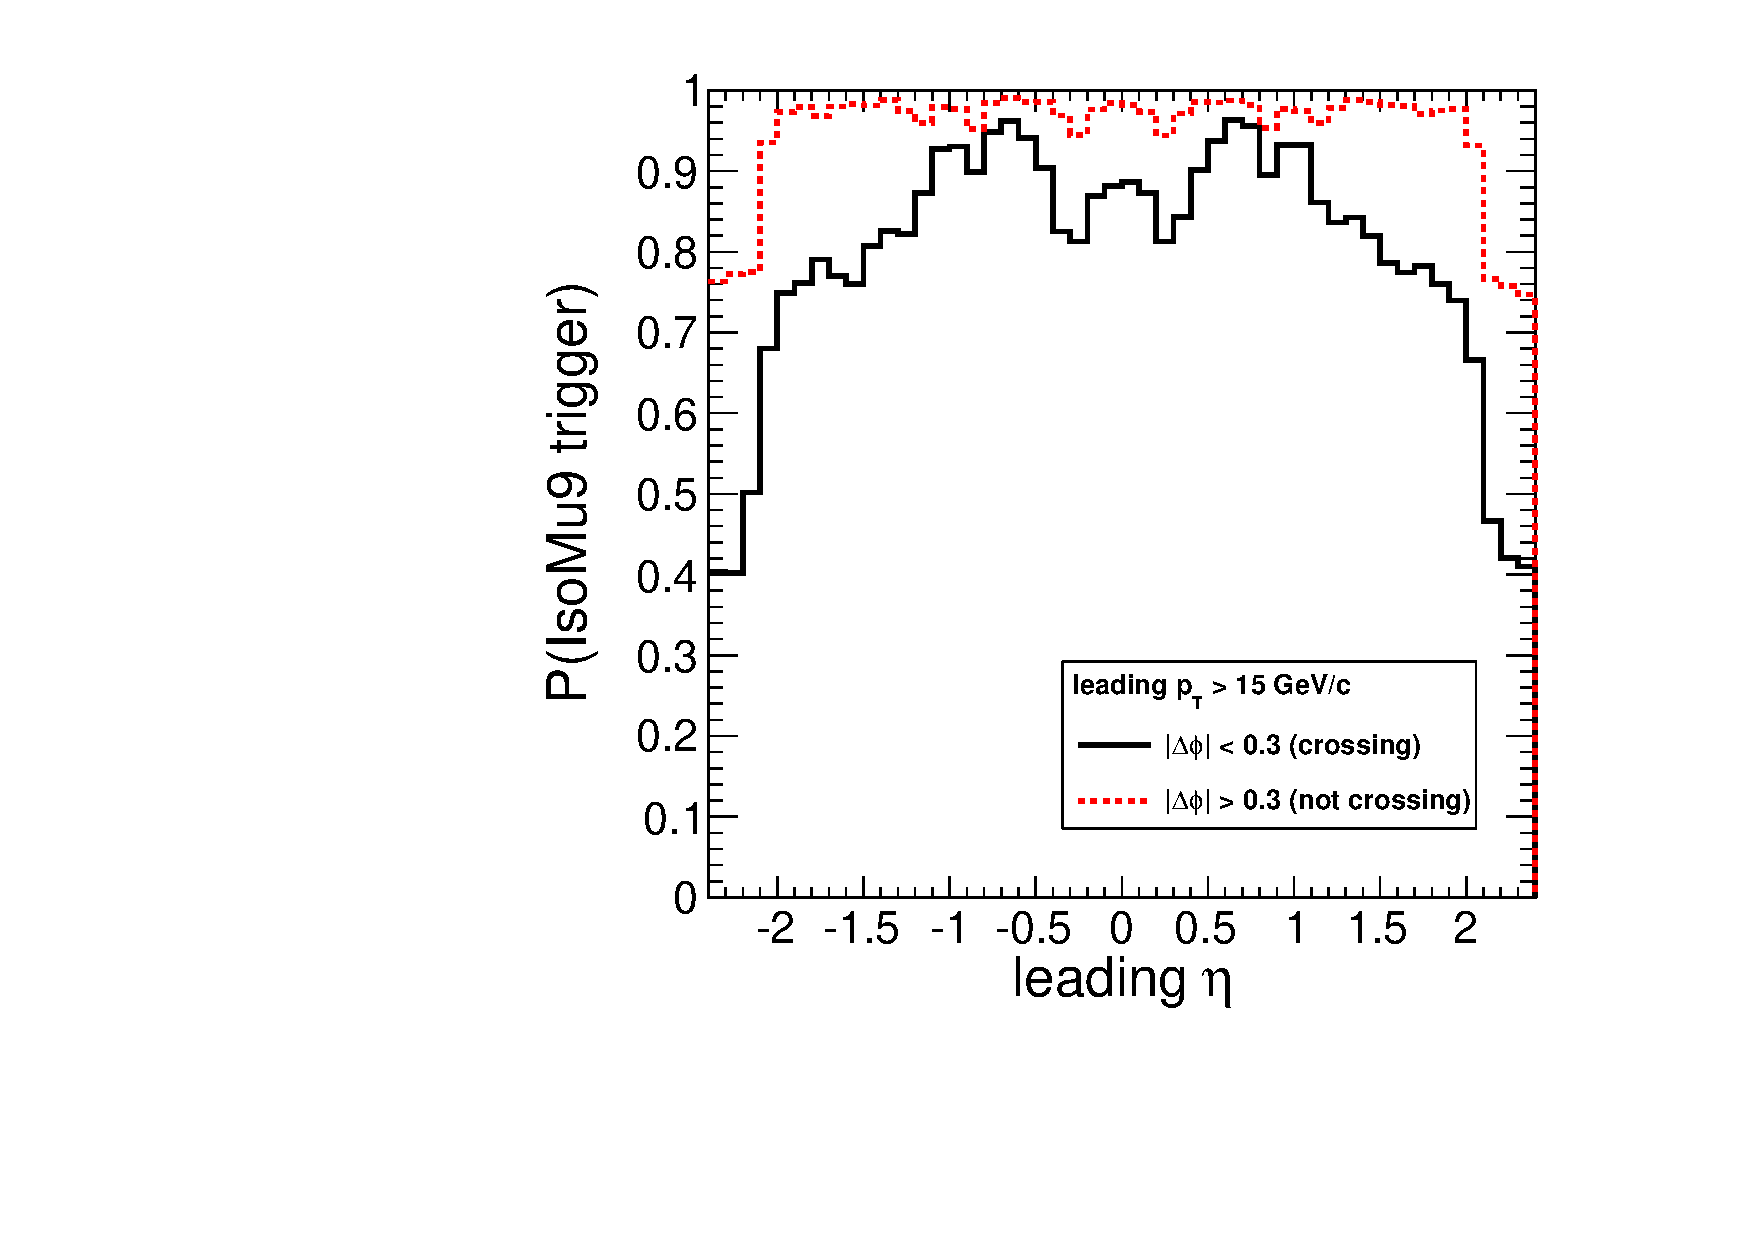
\includegraphics[width=\linewidth]{eta_mass5cut_triggerIsoMu9.pdf}

\column{0.33\linewidth}
\centering double-muon (DMu3)

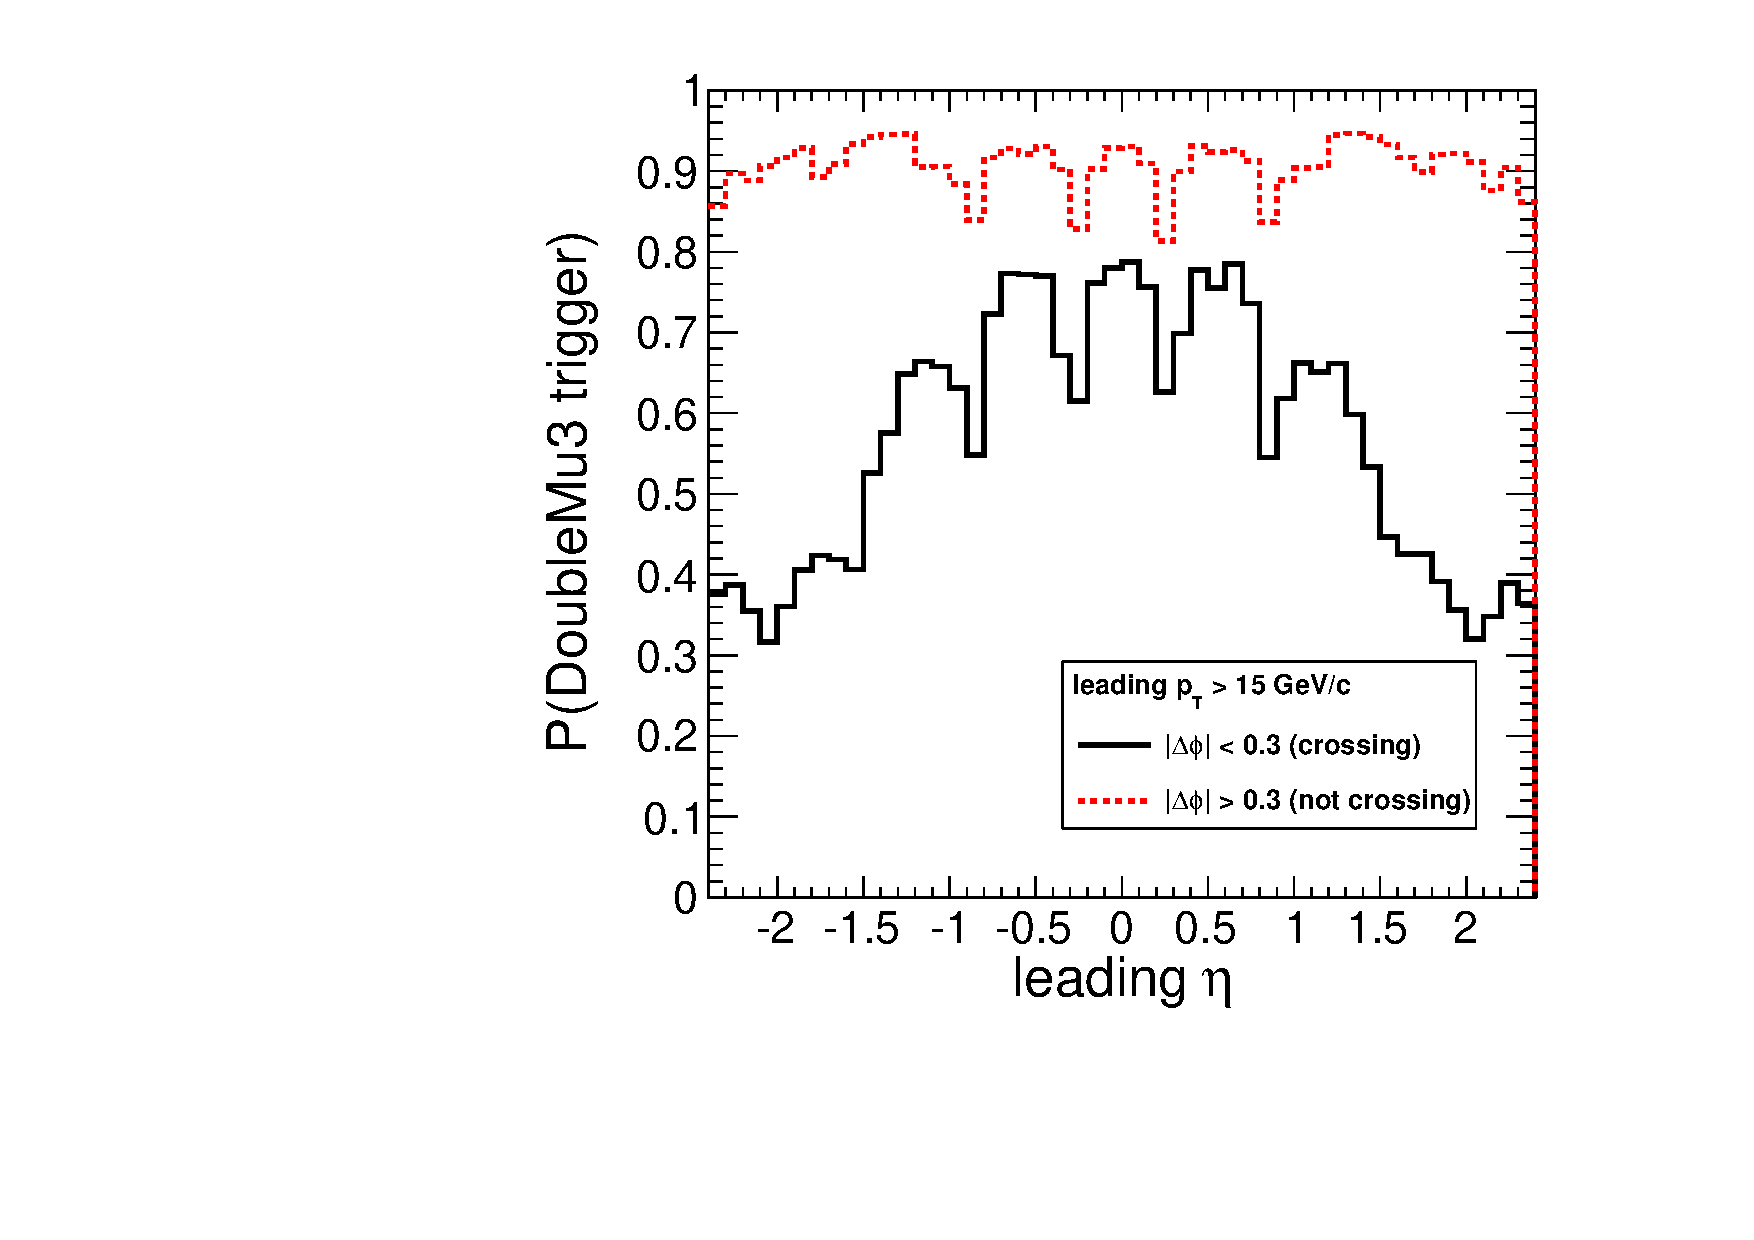
\includegraphics[width=\linewidth]{eta_mass5cut_triggerDoubleMu3.pdf}
\end{columns}

\begin{itemize}
\item Only the single-muon barrel trigger is highly efficient for
  nearby muons, regardless of crossing, so we define acceptance:

each event must have at least one $p_T > 15$~GeV/$c$, $|\eta| < 0.9$ muon
\end{itemize}
\end{frame}

\begin{frame}
\frametitle{Muon reconstruction}

\begin{itemize}
\item GlobalMuons are also inefficient for crossing muons ($\varepsilon \sim 50$\%)
\item TrackerMuons are much less sensitive to crossing, so all muons in the analysis must be:
\begin{itemize}
\item TrackerMuons with at least 2 arbitrated segments,
\item $p_T > 5$~GeV/$c$, $|\eta| < 2.4$,
\item track normalized $\chi^2$ $<$ 4, at least 8 hits.
\end{itemize}

\item Quality TrackerMuon efficiency for crossing and \textcolor{red}{non-crossing} muons:
\end{itemize}

\mbox{ } \hfill 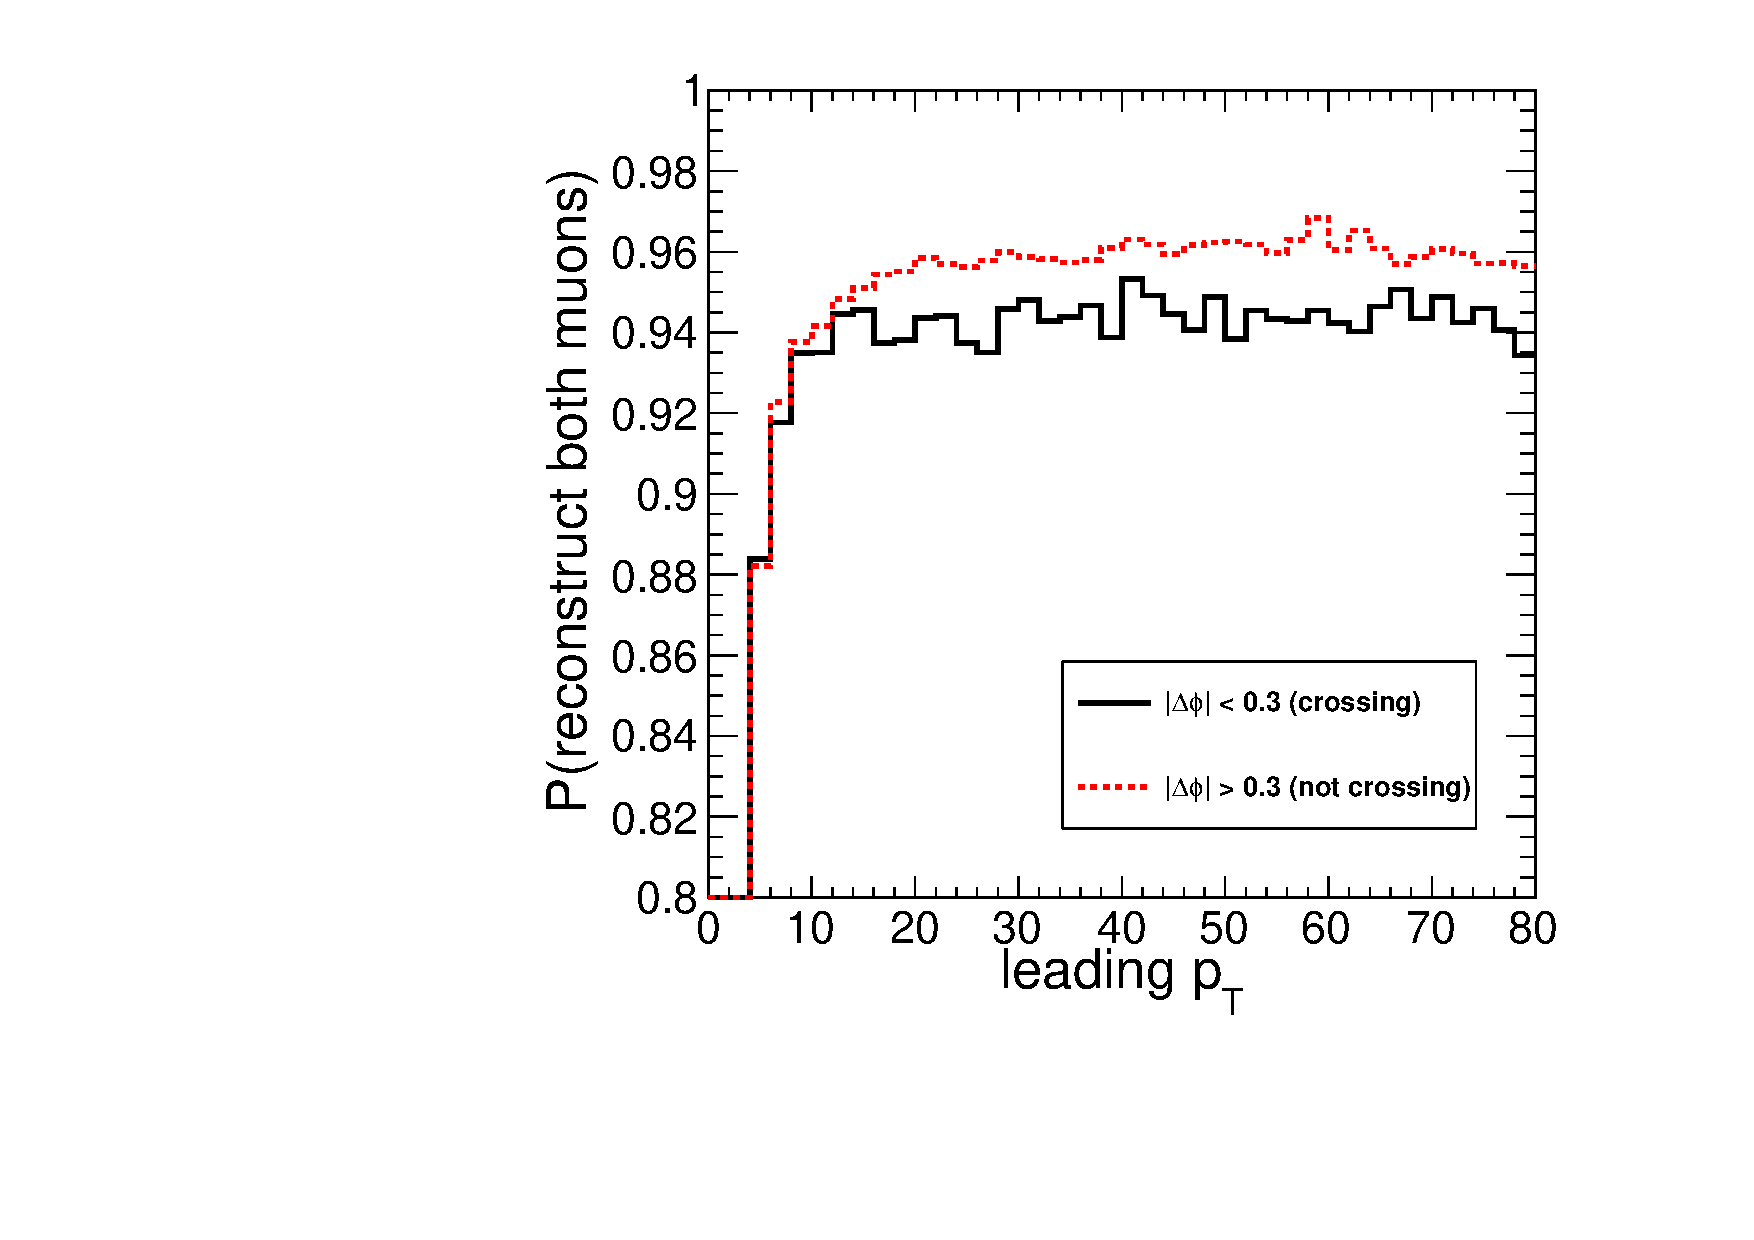
\includegraphics[width=0.4\linewidth]{pt_mass5cut_twoTrackerMuons.pdf} \hfill
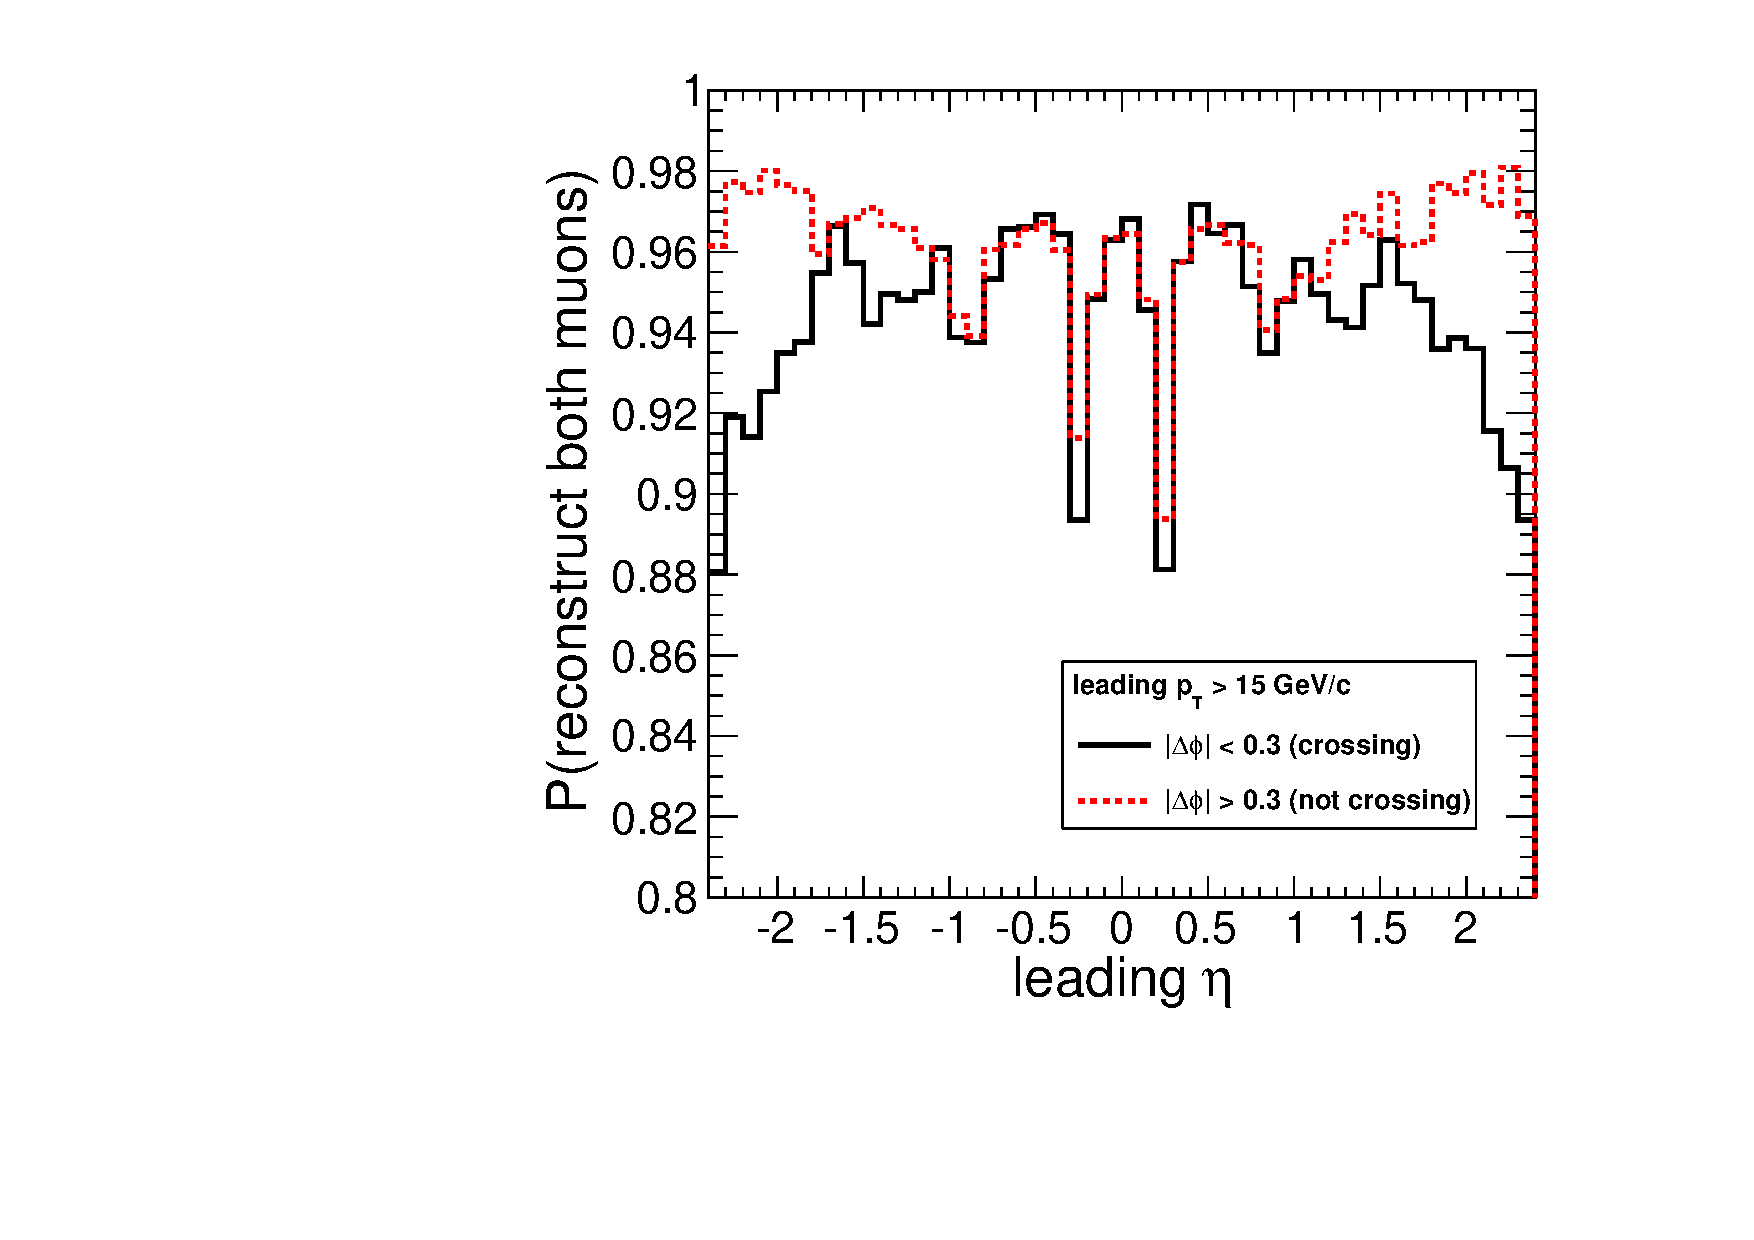
\includegraphics[width=0.4\linewidth]{eta_mass5cut_twoTrackerMuons.pdf} \hfill \mbox{ }
\end{frame}

\section*{Implications for Benchmark Models}
\begin{frame}

\vfill
\begin{center}
\Huge \textcolor{blue}{Implications for Benchmark Models}
\end{center}

\vfill
\end{frame}

\begin{frame}
\frametitle{Benchmark model acceptance}

\vspace{0.5 cm}
\begin{columns}
\column{0.5\linewidth}
\centering SUSY dark matter + extra $\mathcal{U}(1)_\s{dark}$ (inspired by PAMELA)

\vspace{0.1 cm}
$z_d \to 2\mu$ and $h_d \to z_dz_d \to 4\mu$

\vspace{0.1 cm}
$m_{z_d} = 1$~GeV/$c^2$, $m_{h_d} = 3$~GeV/$c^2$

\vspace{0.1 cm}
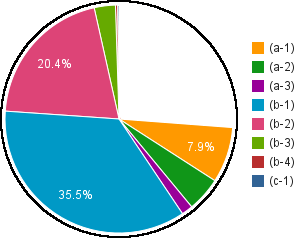
\includegraphics[width=0.6\linewidth]{chart2d_u1.png}

\column{0.5\linewidth}
\centering NMSSM Higgs \\
(inspired by hidden Higgs)

\vspace{0.1 cm}
$h \to aa \to 2\mu, \, 2\mu$

\vspace{0.1 cm}
$m_h = 100$~GeV/$c^2$, $m_a = 2$~GeV/$c^2$

\vspace{0.1 cm}
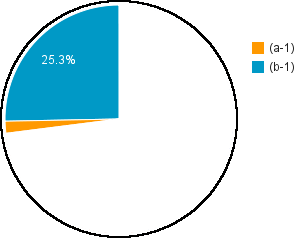
\includegraphics[width=0.6\linewidth]{chart2d_NMSSM.png}
\end{columns}

\begin{itemize}
\item Extra-$\mathcal{U}(1)$ model produces complicated events that
  have high acceptance but fall into many signal regions
{\scriptsize \begin{itemize}
\item (a-1): 1 high-$p_T$ mu-jet with 2 muons
\item (b-1): 2 mu-jets with 2 muons each
\item (b-2): 2 mu-jets: one with 2 muons, the other with 4 muons
\end{itemize}}
\item Because NMSSM is a heavy $\to$ light light model, it produces 2
  well-separated mu-jets, each with exactly 2 muons: (b-1)
\end{itemize}
\end{frame}

\begin{frame}
\frametitle{Benchmark model acceptance}

\begin{itemize}
\item This is the Dark SUSY model used in the Princeton studies
\end{itemize}

\begin{columns}
\column{0.25\linewidth}

\column{0.25\linewidth}
\centering $m_{\tilde{q}} = 200$~GeV/$c^2$

\column{0.25\linewidth}
\centering $m_{\tilde{q}} = 400$~GeV/$c^2$

\column{0.25\linewidth}
\centering $m_{\tilde{q}} = 600$~GeV/$c^2$
\end{columns}

\vspace{0.25 cm}
\begin{columns}
\column{0.25\linewidth}
\mbox{$\tilde{n}_2 \to \tilde{n}_1 \gamma_\s{dark} \to 2\mu$}

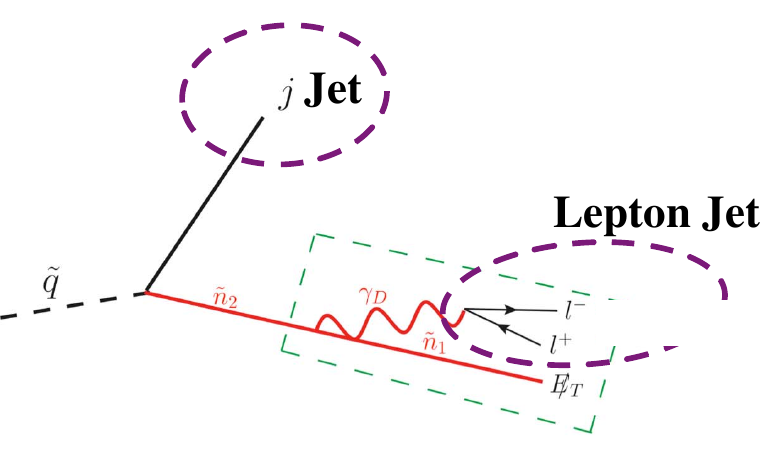
\includegraphics[width=\linewidth]{diagram_squark_2mu.png}

\column{0.25\linewidth}
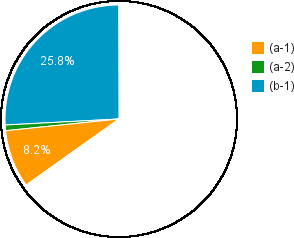
\includegraphics[width=\linewidth]{chart2d_2mu_200.png}

\column{0.25\linewidth}
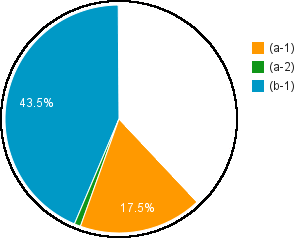
\includegraphics[width=\linewidth]{chart2d_2mu_400.png}

\column{0.25\linewidth}
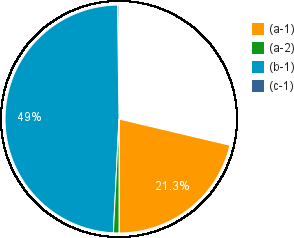
\includegraphics[width=\linewidth]{chart2d_2mu_600.png}
\end{columns}

\vspace{0.25 cm}
\begin{columns}
\column{0.25\linewidth}
\mbox{$\tilde{n}_2 \to \tilde{n}_1 h_\s{dark} \to 4\mu$}

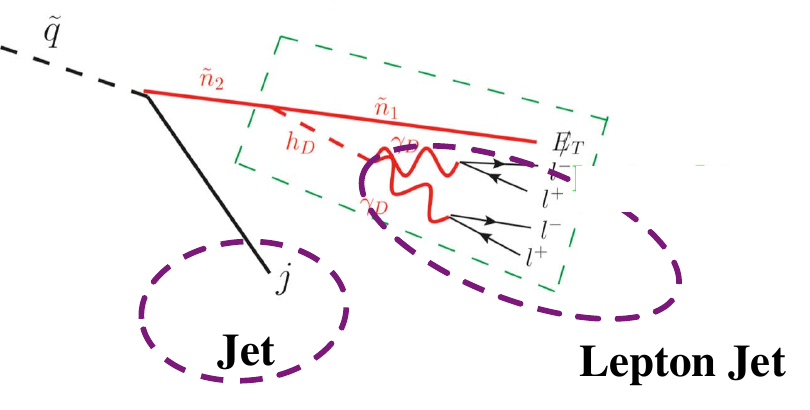
\includegraphics[width=\linewidth]{diagram_squark_4mu.png}

\column{0.25\linewidth}
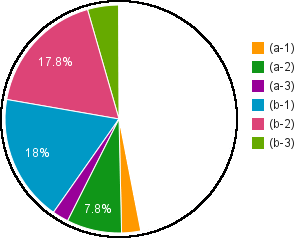
\includegraphics[width=\linewidth]{chart2d_4mu_200.png}

\column{0.25\linewidth}
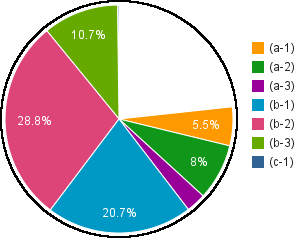
\includegraphics[width=\linewidth]{chart2d_4mu_400.png}

\column{0.25\linewidth}
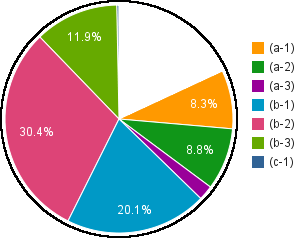
\includegraphics[width=\linewidth]{chart2d_4mu_600.png}
\end{columns}

\vspace{0.3 cm}
\begin{itemize}
\item Increasing $\tilde{q}$ mass doesn't change the topology of
  events, but does increase the overall acceptance
\end{itemize}
\end{frame}

\begin{frame}
\frametitle{Benchmark model acceptance}

\begin{itemize}
\item Hidden sector particles may not have a preference for muons
\begin{itemize}
\item if some decay to electrons or pions, the acceptance would drop
\item but also the event topologies would change
\end{itemize}
\end{itemize}

\vspace{0.5 cm}
\begin{columns}
\column{0.33\linewidth}
\centering $\mathcal{B}(\gamma_\s{dark} \to \mu\mu)$ = 100\%

\vspace{0.2 cm}
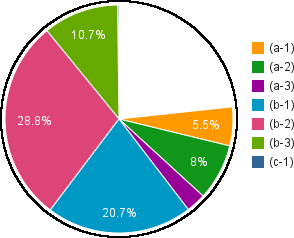
\includegraphics[width=0.9\linewidth]{chart2d_Br100.png}

\column{0.33\linewidth}
\centering $\mathcal{B}(\gamma_\s{dark} \to \mu\mu)$ = 50\%

\vspace{0.2 cm}
\includegraphics[width=0.9\linewidth]{chart2d_Br50.png}

\column{0.33\linewidth}
\centering $\mathcal{B}(\gamma_\s{dark} \to \mu\mu)$ = 33\%

\vspace{0.2 cm}
\includegraphics[width=0.9\linewidth]{chart2d_Br33.png}
\end{columns}

\vspace{0.5 cm}
\begin{itemize}
\item $\mathcal{B} = 100$\%: primarily (b-1) ($2\mu$, $2\mu$) and (b-2) ($2\mu$, $4\mu$)
\item $\mathcal{B} = 33$\%: primarily (a-1) (single dimuon)
\end{itemize}
\end{frame}

%% \section*{First section}
%% \begin{frame}
%% \begin{center}
%% \Huge \textcolor{blue}{First section}
%% \end{center}
%% \end{frame}

\begin{frame}
\frametitle{Limits on Dark SUSY}

\begin{columns}
\column{0.5\linewidth}
\centering \mbox{$\tilde{n}_2 \to \tilde{n}_1 \gamma_\s{dark} \to 2\mu$}

\includegraphics[width=0.7\linewidth]{diagram_squark_2mu.png}

\includegraphics[width=\linewidth]{squarklimits_gamgam.png}

$m_{\tilde{q}}$ [GeV/$c^2$]

\column{0.5\linewidth}
\centering \mbox{$\tilde{n}_2 \to \tilde{n}_1 \gamma_\s{dark} \to 2\mu$}

\includegraphics[width=0.7\linewidth]{diagram_squark_2mu.png}

\includegraphics[width=\linewidth]{squarklimits_hh.png}

$m_{\tilde{q}}$ [GeV/$c^2$]
\end{columns}
\end{frame}

\begin{frame}
\frametitle{Conclusions}

\begin{itemize}\setlength{\itemsep}{0.5 cm}
\item High mass scale of the LHC presented a new opportunity to
  discover or constrain a general class of hidden valley models

\item We cast a wide net for discovery: any model that produces
  several on-shell resonances per event {\bf or} one high-$p_T$
  resonance, decaying inclusively to muon pairs

\item No events were found compatible with several resonances per
  event; high-$p_T$ spectrum is compatible with the Standard Model

\item Many different signal regions made this a complicated analysis!

\item To put the sensitivity of these results into concrete terms, we
  set limits on three benchmark models
\end{itemize}

\label{numpages}
\end{frame}

\section*{Backup: Understanding the Low-Mass Dimuon Spectrum}
\begin{frame}
\vspace{0.75 cm}
\begin{center}
\Huge \textcolor{blue}{Backup: Understanding the Low-Mass Dimuon Spectrum}

\vspace{0.25 cm}
\includegraphics[width=0.75\linewidth]{dimuonSpectrum_40pb-1.pdf}
\end{center}
\end{frame}

\begin{frame}
\frametitle{Low-mass dimuons}

\vspace{0.25 cm}
\hfill \includegraphics[width=0.5\linewidth]{support_mass_all.pdf}

\vspace{-3.7 cm}
\begin{itemize}
\item ``Raw'' mass spectrum has \\ several components:
\begin{itemize}
\item resonances (prompt and \\ from $b$ decays)
\item double-semileptonic \\ $b \to \mu\mu X$ continuum
\item low-mass Drell-Yan
\end{itemize}

\item MC isn't perfect: study data/MC differences using isolation (defined
  such that $\mu\mu$ doesn't self-veto) and distance of flight ($L_{xy}$)
\end{itemize}

\includegraphics[width=0.5\linewidth]{support_iso_lowmass.pdf}
\includegraphics[width=0.5\linewidth]{support_lxy_continuum.pdf}
\end{frame}

\begin{frame}
\frametitle{Low-mass dimuons}

\begin{itemize}
\item Split sample into $b\bar{b}$ and Drell-Yan/prompt resonances with this cut:

\mbox{ } \hfill $Iso > 4.5$~GeV/$c$ {\bf or} $L_{xy} > 2$~mm \hfill \mbox{ }
\label{pag:bbcuts}
\end{itemize}

\includegraphics[width=0.5\linewidth]{support_mass_antibbbar.pdf}
\includegraphics[width=0.5\linewidth]{support_mass_bbbar.pdf}

\begin{itemize}
\item Much of the low-mass spectrum is Drell-Yan (not in any official samples, so we generated it with Pythia 8)
\item Some resonances are not in inclusive-muon MC: $\omega(782)$, $\psi'(3686)$
\item There's also a low-mass excess \textcolor{red}{(red circle),} too wide to be a resonance peak, and too low in mass to be $\eta \to \mu\mu\gamma$
\end{itemize}
\end{frame}

\begin{frame}
\frametitle{Low-mass dimuons}

\hfill \includegraphics[width=0.45\linewidth]{lxyresolution.pdf}

\vspace{-3.7 cm}
\begin{itemize}
\item Part of the explanation: the cut

$Iso > 4.5$~GeV/$c$ {\bf or} $L_{xy} > 2$~mm

depends on $L_{xy}$, which becomes \\ imprecise for nearly collinear \\
tracks: Drell-Yan leaks into the \\ ``$b\bar{b}$'' sample

\item This mass region is below the \\ Pythia generator-level mass
  cut-off\ldots

\item About 1/10$^\s{th}$ of what remains passes $Iso > 4.5$~GeV/$c$
  alone: misreconstructed Drell-Yan?

\item History of this study is a geometric progression of explaining 90\%, then explaining 90\% of what's left, etc..
\end{itemize}
\end{frame}

\end{document}
